\chapter{Charge Readout Planes}
\label{ch:fddp-CRP}

%%%%%%%%%%%%%%%%%%%%%%%%%%%%%%%%%%%%%%%%%%%%%%%%%%%%%%%%%%%%%%%%%%%%
\section{Charge Readout Planes (CRP) Overview}
\label{sec:fddp-crp-ov}


%%%%%%%%%%%%%%%%%%%%%%%%%%%%%%%%%
\subsection{Introduction}
\label{sec:fddp-crp-intro}

In the \dual \lartpc concept, the ionization electrons are multiplied in avalanches  occurring inside micro-pattern detectors, the \dwords{lem}, located in the argon gas phase above the \lar %level. 
surface. The drift field of the TPC brings the electrons up to the \lar surface where they can  be    extracted into the gas using a 
\SI{2}{kV/cm} \efield defined across the liquid-gas interface.

This extraction field is defined by the potentials applied to submersed extraction grid (stainless steel wires tensioned in both $x$ and $y$ directions) and to the bottom side of the \dwords{lem}. The \dwords{lem} are printed circuit boards oriented horizontally, with conductive layers (electrodes) on the top and bottom surfaces, and many holes drilled through.  The holes form a micro-pattern structure within which the amplification occurs given the presence of a strong \efield.

By applying voltages across the two electrodes of the \dword{lem}, an \efield region (up to \SI{35}{kV/cm}) is defined in the holes, which produces an electronic signal gain exceeding \num{20} after the initial phase of charging-up the \dword{lem} dielectric material.  Electrons transiting these high \efield regions in the holes trigger Townsend multiplication in the pure argon gas.

The amplified charge is then collected and recorded on a \twod anode consisting of two sets of \dpstrippitch-pitch gold-plated copper strips that provide the $x$ and $y$ coordinates (and thus two orthogonal views) of the event. The strips are defined by a pattern of tracks on the bottom face of the anode printed circuit board. It is possible  to define two electrically insulated views of strips crossing each other orthogonally by ensuring continuity of the tracks with a set of vias and tracks extending to the top face of the anode printed circuit board.

Typical \efield{}s between each stage of the readout are
illustrated in Figure~\ref{fig:setup}. Table~\ref{tab:crp_dist} shows the inter-stage distance and the tolerances required to obtain uniformity of gain to within $\sim$5\%.

\begin{dunefigure}[Dual-phase readout]{fig:setup}
{Illustration of the \efield{}s in the amplification region of a \dual \lartpc. The simulated field lines in dark blue indicate the paths followed by the drifting charges (without diffusion).}
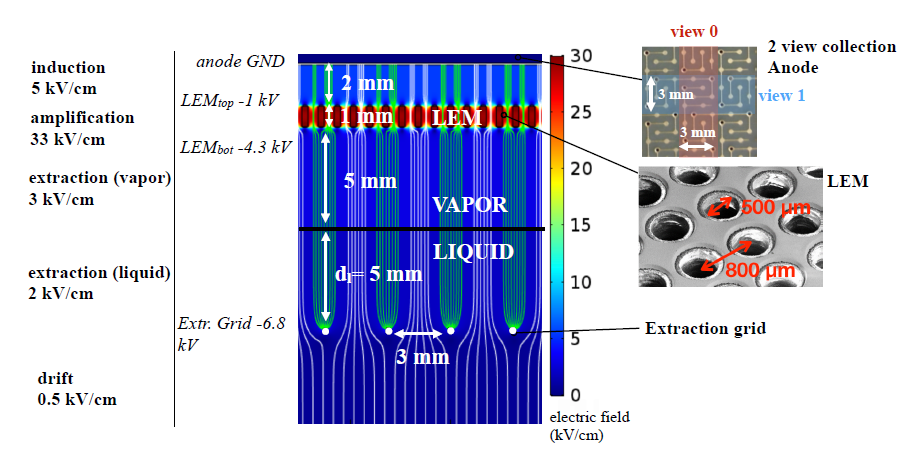
\includegraphics[width=.85\textwidth]{amplification-principle2.png}  
\end{dunefigure}
\begin{dunetable}[Interstage distances and \efield settings of the \dual readout components]{lp{2cm}p{2cm}l}{tab:crp_dist}{Interstage distances and \efield settings of the \dual readout components.} 
 Component & Distance [mm] & Tolerance [mm] & \efield [kV/cm]  \\ \toprowrule
 Anode-\dword{lem} top electrode  & \num{2} & \num{0.1} & \num{5}\\ \colhline
 \dword{lem} top-bottom electrode   & \num{1} & \num{0.01} & \numrange{30}{35}\\ \colhline
 \dword{lem} bottom electrode-grid        &\num{10} & \num{1} & \num{2} (in \lar) and \num{3} (in gaseous argon)\\
 \end{dunetable}

The extraction grid, \dword{lem} and anode are assembled into three-layered \textit{sandwiches} with precisely defined inter-stage distances and inter-alignment,  which are then connected together horizontally into modular units of area \SI{9}{m$^2$}. These units are called \dwords{crp}. Figure~\ref{fig:figure-label-crp} shows an 
engineering view of one \dword{crp} fully assembled.

\begin{dunefigure}
[View of a complete  \SI{9}{m$^{2}$} \dword{crp} module]
{fig:figure-label-crp}
{View of a complete  \SI{9}{m$^{2}$} \dword{crp} module.}
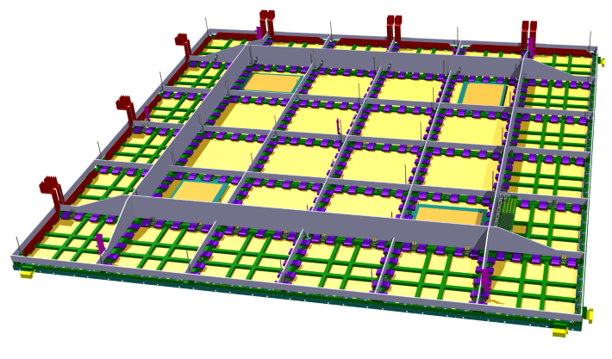
\includegraphics[width=0.75\textwidth]{CRP-fig1.png}
\end{dunefigure}

The \dword{crp} mechanical structure provides the integration of the \dword{lem}-anode sandwiches over a large area by minimizing the dead spaces. The planarity of the active surface must be guaranteed despite possible sagging effects with respect to the three hanging points, differential thermal contraction effects on the various  components and the presence of a temperature gradient in the gas phase, which could induce different thermal contractions as a function of the distance from the liquid surface. In order to %solve these aspects 
ensure the planarity, the design % is based on 
incorporates a supporting frame in Invar, which % . Invar allows building 
can provide a stiff supporting structure, extending vertically into the gas phase, with little sagging and %little 
very minor contraction effects. The \dword{lem} and anodes, which would be affected by a significant thermal contraction, are integrated into a G10 planar structure with similar contraction %effects. 
properties. The G10 structure is mechanically decoupled on the horizontal plane with respect to the Invar structure  and it is free to slide during thermal contraction. 

%%%%%%%%%%%%%%%%%%%%%%%%%%%%%%%%%%%%%
\subsection{Design Considerations}
\label{sec:fddp-crp-des-consid}

Each \dword{crp} is an independent detector element that performs charge
extraction, multiplication and collection, and has its own \dword{hv} system and independent signal \fdth{}s. The entire area of the \dword{lem} and anode in a \dword{crp} is active. The position and the parallelism with respect to the \lar surface can be individually adjusted for each \dword{crp}.

The \dword{lem} and corresponding anode are mounted in units of \num{50}$\times$\SI{50}{cm$^2$}, called %\dword{lem}/Anode Sandwich (LAS) 
\dword{las} modules, before being assembled with an extraction grid into a \dword{crp}. Each anode in a \dword{las} is segmented in 50-cm long $x$ and $y$ strips . Adjacent \dword{las} anodes are bridged together to form readout strips of the required length by connecting short flat cables to KEL\footnote{KEL 8925E-068-1795 .27mm Pitch, 2 piece, IDC for 0.635mm FC Connector, Low profile type, KEL Corporation\texttrademark{}, \url{https://www.kel.jp/english/product/}.} connectors soldered onto the top sides of the anodes. The signals from the last anode in each  strip chain are brought to \fdth{}s mounted on the other side of the front-end electronics embedded inside dedicated signal-\fdth chimneys using \SI{50}{cm}-long flat cables.

Each \dword{crp} is independently hung from the vessel deck through its three
suspension \fdth{}s. It has its own \dword{hv} system and  independent signal and slow-control \fdth{}s.

Table~\ref{tab:crpphysicsparams} summarizes the set of requirements and parameters that drive the \dwords{crp} design. 

\begin{dunetable}
[Important parameters for the \dword{crp} system design]
{p{0.8\textwidth}}
{tab:crpphysicsparams}
{Important parameters for the \dword{crp} system design}   
Parameter \\ \toprowrule
 Planarity tolerance on the detection plane over \num{3}$\times$\SI{3}{m$^{2}$}  $\pm$\SI{0.5}{mm} \\ \colhline
 \dword{crp} vertical positioning precision  $\pm$\SI{0.5}{mm} \\ \colhline
 Range of vertical displacement is $\pm$\SI{20}{mm}\\ \colhline
 Lateral inter \dword{crp} dead space  less than \SI{10}{mm} \\\colhline
 Distance between the extraction grid wires and the \dword{lem} plane: 10mm\\ \colhline 
 \dword{hv} of the extraction grid wires in \lar:  \SI{6.8}{kV} \\ \colhline
 \dword{hv} of the \dword{lem} down surface in gas argon:  \SI{4.5}{kV}\\ \colhline
 \dword{hv} of the \dword{lem} up surface in gas argon: \SI{1}{kV}\\ \colhline
\end{dunetable}

The \dword{crp} design foreseen for the \dword{dpmod} is based on the one developed for \dword{pddp}.

%%%%%%%%%%%%%%%%%%%%%%%%%%%%%%%%
\subsection{Scope}
\label{sec:fddp-crp-scope}

The scope of the \dwords{crp} includes the continued procurement of materials for, and the fabrication, testing, delivery and installation of the following systems: 

\begin{itemize}
\item  Production and \dword{qa} of the \dword{lem} and anodes;
\item  Production of the G10 and Invar frames;
\item Production of the suspension \fdth{}s and motorization;
\item Production of the extraction grid elements;
\item Production of the HV distribution system associated to the \dword{crp} to apply voltages to the \dword{lem} and anodes;
\item Production of the system of temperature probes associated to the \dword{crp};
\item Production of the system of level meters associated to the \dword{crp};
\item Production of the system to pulse the strips associated to the \dword{crp};
\item Production of the transportation and storage boxes for the \dwords{crp};
\item Assembly of the \dwords{las};
\item Assembly of the \dword{crp} structures, \dwords{las}  grid elements, \dword{hv}, slow controls and cabling for each \dword{crp};
\item Testing of the assembled \dwords{crp};
\item Installation in the storage boxes of the produced \dwords{crp};
\item Installation in the transportation boxes and delivery of the \dwords{crp} to \surf{}; % to be installed;
\item Installation, cabling and test of the \dwords{crp} in the cryostat.
\end{itemize}


%%%%%%%%%%%%%%%%%%%%%%%%%%%%%%%%%%%%%%%%%%%%%%%%%%%%%%%%%%%%%%%%%%%%
\section{CRP Design}
\label{sec:fddp-crp-design}

The complete \dword{crp} system includes, as illustrated in Figure~\ref{fig:figure-label-crp2}:
\begin{itemize}
\item Mechanical frames  ;
\item The detection plane made of \dwords{lem} and anodes ;
\item The extraction grid;
\item Instrumentation devices: level meters, distance meters, temperature probes;
\item Internal cabling: to patch panels (\dword{lem} \dword{hv}, slow control instruments);
\item Suspension and control system.
\end{itemize}

\begin{dunefigure}[Main components of a \dword{crp} module of  \SI{9}{m$^{2}$}]{fig:figure-label-crp2}
{Main components of a \dword{crp} module of  \SI{9}{m$^{2}$}}
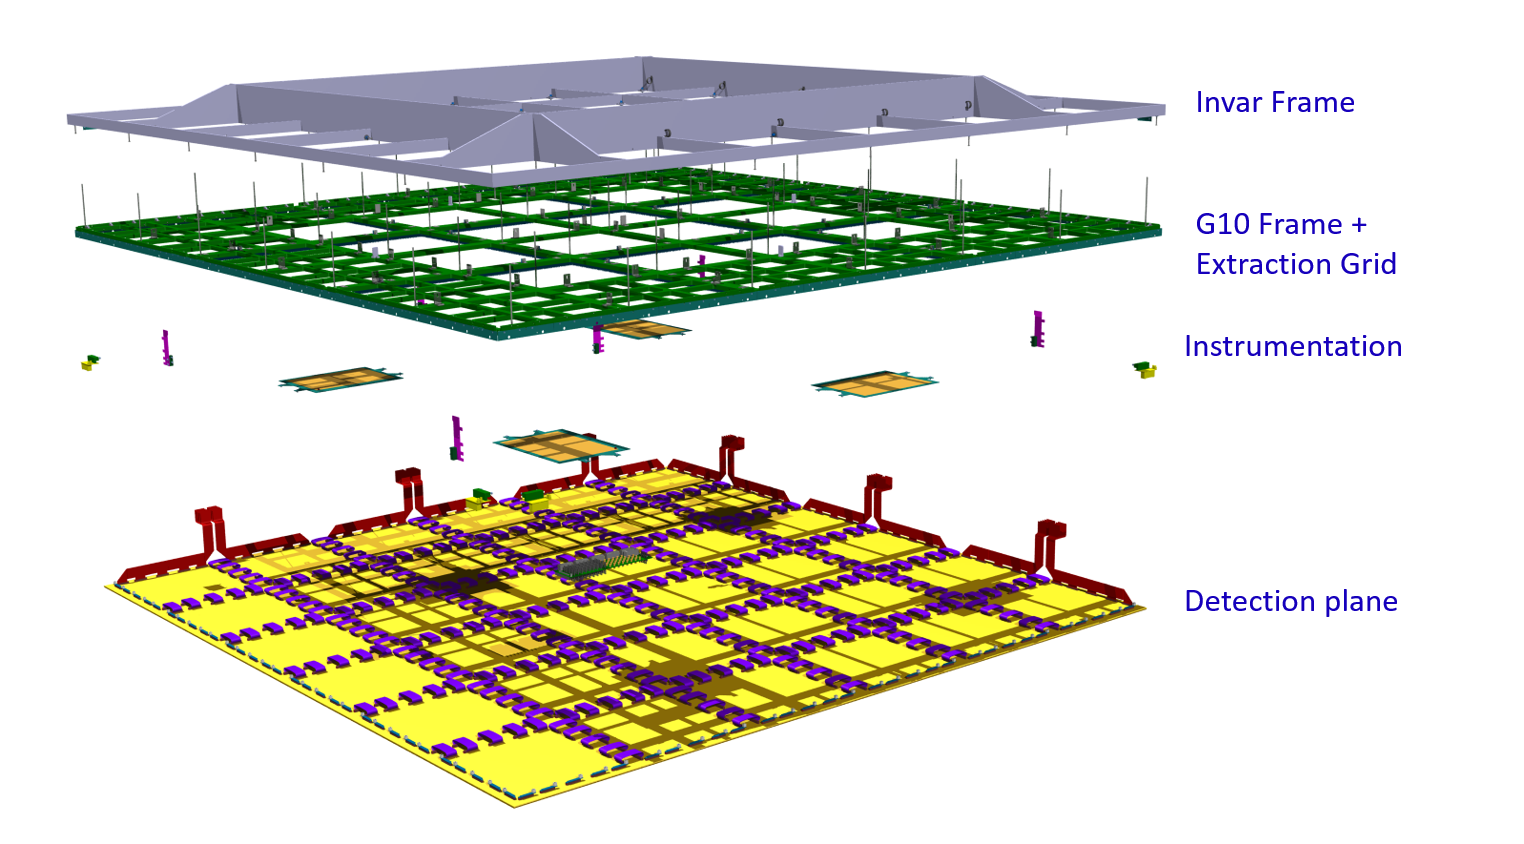
\includegraphics[width=0.8\textwidth]{CRP-fig2.png}
\end{dunefigure}

%%%%%%%%%%%%%%%%%%%%%%%%%%%%%%%%%%%
\subsection{Mechanical structure}
\label{sec:fddp-crp-mechanics}
%%%%%%%%%%%%%%%%%%%
\subsubsection{Invar Frame}

The main mechanical supporting structure of the \dword{crp} is made of Invar nickel-iron alloy. This material is chosen for its low coefficient of thermal expansion leading to a very small deformation at cold temperatures, especially in the gas argon where the temperature gradient in the cryostat may be of the order of a few \si{K/cm}.
The structure is made of a grid of soldered Invar beams \SI{3000}{mm} long and \SI{6.5}{mm} wide. The four main ones have a height of \SI{150}{mm} while the internal ones are \SI{40}{mm} height as well as the four surrounding plates. The heights have been optimized to keep the stiffness as needed and to reduce the total frame weight pf %which amounts to
 about \SI{112}{kg}.
Figure~\ref{fig:invarframe} shows the soldering of one of the first \dword{crp} frame for \dword{pddp}.

\begin{dunefigure}[First \dword{crp} Invar frame under construction for \dword{pddp}]{fig:invarframe}
{First \dword{crp} Invar frame under construction for \dword{pddp}}
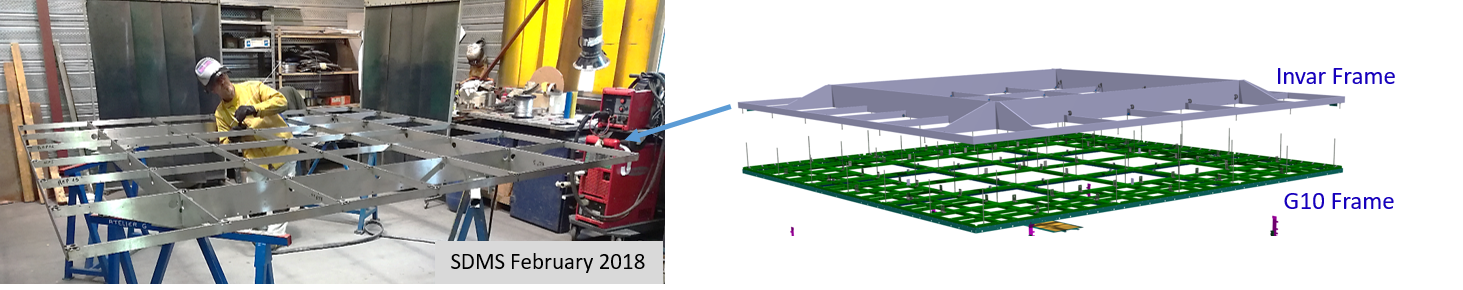
\includegraphics[width=0.95\textwidth]{invar-framev2.png}
\end{dunefigure}

\subsubsection{G10 Frames and Modules}
\label{sec:invar-frame}

The \num{3}$\times$\SI{3}{m$^{2}$}  G10 fiberglass structure used to attach the \num{36} \dwords{lem} and anodes, the extraction grid and the level meters is composed of an assembly of nine \num{1}$\times$\SI{1}{m$^{2}$} subframes. The choice of G10 is driven by the need to match the \dword{lem} and anode thermo-mechanical behavior and avoid over-stress due to differential thermal contraction. 
Figure~\ref{fig:crp-g10} shows the pattern of the nine G10 parts composing a full \dword{crp} frame as well as the supporting comb positioned at every meter, and the extraction grid support plates along the side of the \dword{crp}.

\begin{dunefigure}[G10 elements of a full \dword{crp} module]{fig:crp-g10}
{G10 elements of a full \dword{crp} module}
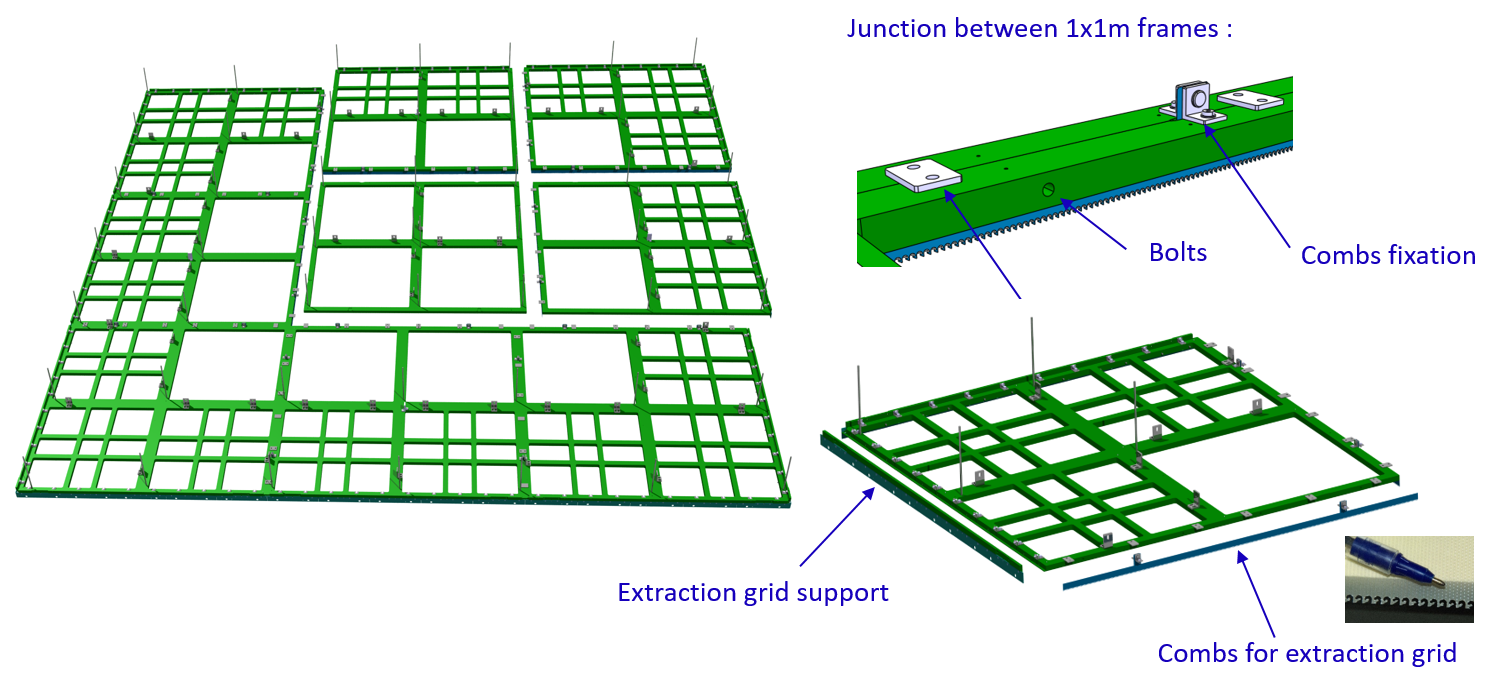
\includegraphics[width=0.8\textwidth]{G10.png}
\end{dunefigure}

Since G10 is a composite material created by stacking multiple layers of glass fibers,  the orientation of the stacking has to be taken into account prior to assembly.
At the construction level, the fiber directions are matched between the different subframes to ensure harmony in thermal shrinkage. Three different patterns have to be produced, one for the four angles, one for the four face centers and one for the central subframe.
Two versions of each pattern for the supporting extraction grid bars and the combs follow same rule.

%The design of the subframes have been calculated 
The subframes have been designed to guarantee %enough 
adequate stiffness in the  regions subject to larger tension while minimizing material in order to reduce the weight.
The G10 structure is \SI{15}{mm} thick and weights about \SI{68}{kg}. 

\subsubsection{Decoupling system}
%During cooling, Invar is nearly keeping its dimensions while G10 frame and \dwords{lem}/Anodes are contracting in similar ways. 
During cooling, Invar's dimensions remain nearly unchanged whereas the G10 frame and \dwords{lem}-anodes contract in similar ways. Thermal decoupling allows a lateral sliding of the G10 frame, without changing the level. 
%\fixme{altitude? maybe `level' is better?}
Dedicated decoupling systems are installed at each corner of the Invar frame (\num{50} systems by  \num{3}$\times$\SI{3}{m$^{2}$} module). One decoupling system that allows the G10+ \dword{lem}-anodes elements to slide is shown in  Figure~\ref{fig:crp-decoupling}.

\begin{dunefigure}[Decoupling system attached to the Invar frame]{fig:crp-decoupling}
{Decoupling system attached to the Invar frame, with detailed view. Example of one of the systems built for \dword{pddp}.}
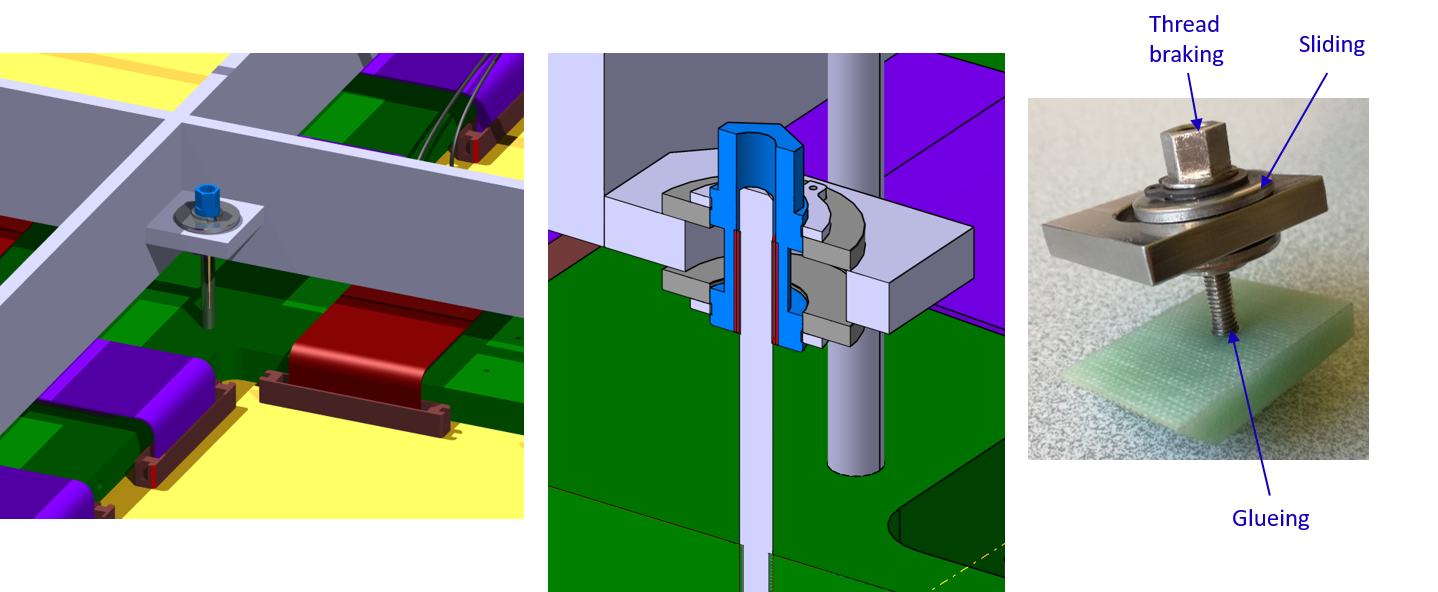
\includegraphics[width=0.8\textwidth]{decoupling.png}
\end{dunefigure}

The full weight of a \dword{crp} including the mass of \dwords{lem} and anodes is about \SI{330}{kg}.

%%%%%%%%%%%%%%%%%%%%%%%%%%%%%%%%%%%
\subsection{Extraction Grid}
\label{sec:fddp-crp-grid}
The extraction grid consists of \SI{100}{\micro\meter}-diameter stainless steel wires tensioned in both $x$ and $y$ directions over the entire \SI{3}{m} length and width of the \dword{crp} with \dpstrippitch pitch. They are soldered into groups of \num{64} on independent wire-tensioning pads oriented perpendicularly to the side of the \dword{crp} frame. Each wire-tensioning pad consists of a printed circuit board (PCB)  that is fixed very precisely to mechanical support beams screwed to the G10 frame of the \dword{crp}, as shown in Figure~\ref{fig:grid-parts}.
 
\begin{dunefigure}[Extraction grid components on the \dword{crp} structure]{fig:grid-parts}
{Extraction grid components on the \dword{crp} structure. On the left are the PCB plates and their supporting bars. On the right is the %system to guarantee the proper 
wire tensioning system with the pushing screws and calibrated wedges to keep the right distance.}
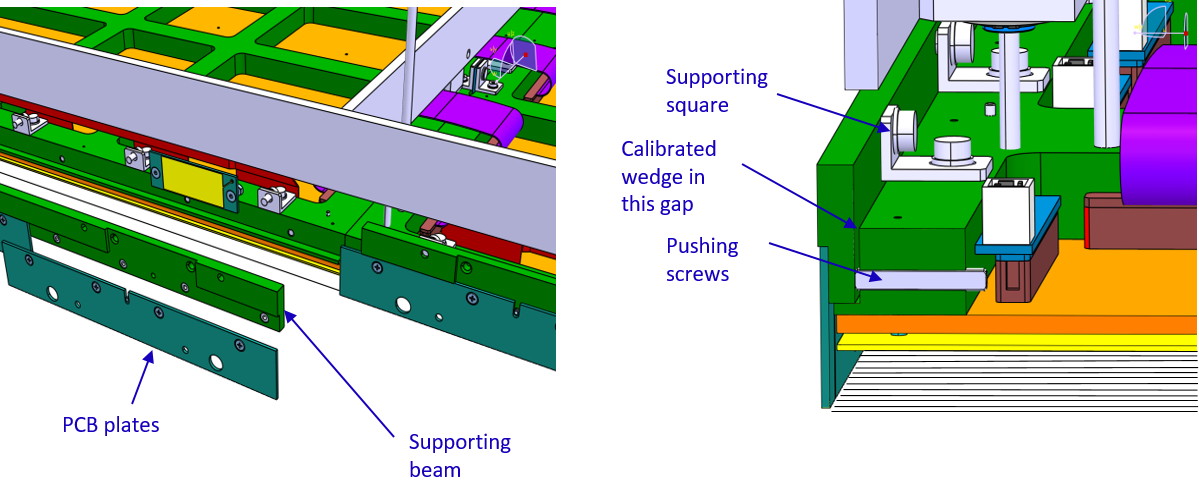
\includegraphics[width=0.8\textwidth]{grid-parts.png}
\end{dunefigure}

The PCB has \num{64} soldering pads with \SI{200}{\micro\meter} grooves for precise positioning of the wires. During the %wire-
soldering process each wire is tensioned and positioned in a groove. The PCB is then mounted on the G10 supporting bars and the tension of the group of \num{64} wires can be precisely adjusted by pushing the supporting bars against the \dword{crp}s G10 frame with screws. The tensioning is performed by tightening \textit{pushing screws}, adding a calibrated wedge, and locking the supporting square.
%The wires, \SI{3}{m} long in both $x$ and $y$ directions, have their sags minimized to \SI{0.1}{mm} thanks to $x$ and $y$ oriented supporting comb-teeth blades  inserted between G10 subframes of 1 m$^2$ size. 
Supporting comb-teeth blades that are inserted between the \SI{1}{m$^2$} G10 subframes in both $x$ and $y$ restrict the sag to \SI{0.1}{mm} in the wires, which are \SI{3}{m} long in both directions. The array of blades penetrates the liquid surface and has the additional benefit of acting as a baffle against potential surface waves in the \lar.

The grid \dword{hv}-connection for a \dword{crp} is made through a varnished copper track into two of the \dword{crp}'s \num{60} PCB plates; a special isolated connection %performed 
is made inside the \dword{crp} structure.

%%%%%%%%%%%%%%%%%%%%%%%%%%%%%%%%%%%
\subsection{Large Electron Multiplier (LEM)}
\label{sec:fddp-crp-lem}

Each \dword{lem} consists of a \SI{1}{mm}-thick,  \num{50}$\times$\SI{50}{cm$^{2}$} copper-clad standard PCB epoxy plate. Holes of \SI{500}{\micro\meter} diameter, through which electrons undergo amplification, are mechanically drilled in a hexagonal pattern with a pitch of \SI{800}{\micro\meter}, yielding about \num{180} holes per \si{cm$^2$}. In addition, each hole has a  \SI{40}{\micro\meter} dielectric rim, obtained by a chemical process, to prevent electrical discharges from occurring near the holes. The holes provide confinement for the UV photons produced during the avalanche process and thus act as a mechanical quencher to prevent photon feedback. This property makes the \dword{lem} suitable for operation in ultra-pure argon vapor without the addition of a quenching gas. The final gold-plated copper thickness of each \dword{lem} electrode is about  \SI{60}{\micro\meter}. Twenty peripheral and nine central \SI{2.2}{mm}-diameter holes are used for assembling the \dword{lem} module together with its anode on the G10 frame. Figure~\ref{fig:LEM_CFR-35} shows a picture of a \dword{lem} module used for  \dword{pddp}. To prevent \dword{hv} discharges near or across the edges, the \dword{lem} module has a  \SI{10}{mm} border free from metallization and another \SI{5}{mm} copper guard ring. Similar copper guard rings are located around the \SI{2.2}{mm} diameter holes and the \dword{hv} connectors. The latter are made with \SI{1.2}{mm} diameter male pins (Deutsch\footnote{Deutsch\texttrademark{} \url{http://www.deutsch.net/}.} 6860-201-22278.) that are soldered onto specifically designed pads imprinted on the \dword{lem} electrodes. The pins are insulated with circular tubes made in MACOR and a  \SI{10}{mm} circular clearance around each pin. 

The total active area of a \dword{lem} module used for  \dword{pddp} represents about \SI{86}{\%} of the \num{50}$\times$\SI{50}{cm$^{2}$} area. The choice of the \dword{lem} design for  \dword{pddp} was made in order to achieve stable operation conditions up to \SI{3.5}{kV} in \dual \lar (D\lar{}) mode, corresponding to amplification gains larger than \num{30} (\num{100}) after (before) charging-up of the \dword{lem} dielectric material. For the \dword{dpmod}, a further optimization of the current \dword{lem} design will  be performed in order  to find the best compromise between the detector active area and the operation stability.

\begin{dunefigure}
[Picture of a \dword{lem} module used for  \dword{pddp}]
{fig:LEM_CFR-35}
{Picture of a \dword{lem} module used for  \dword{pddp}}
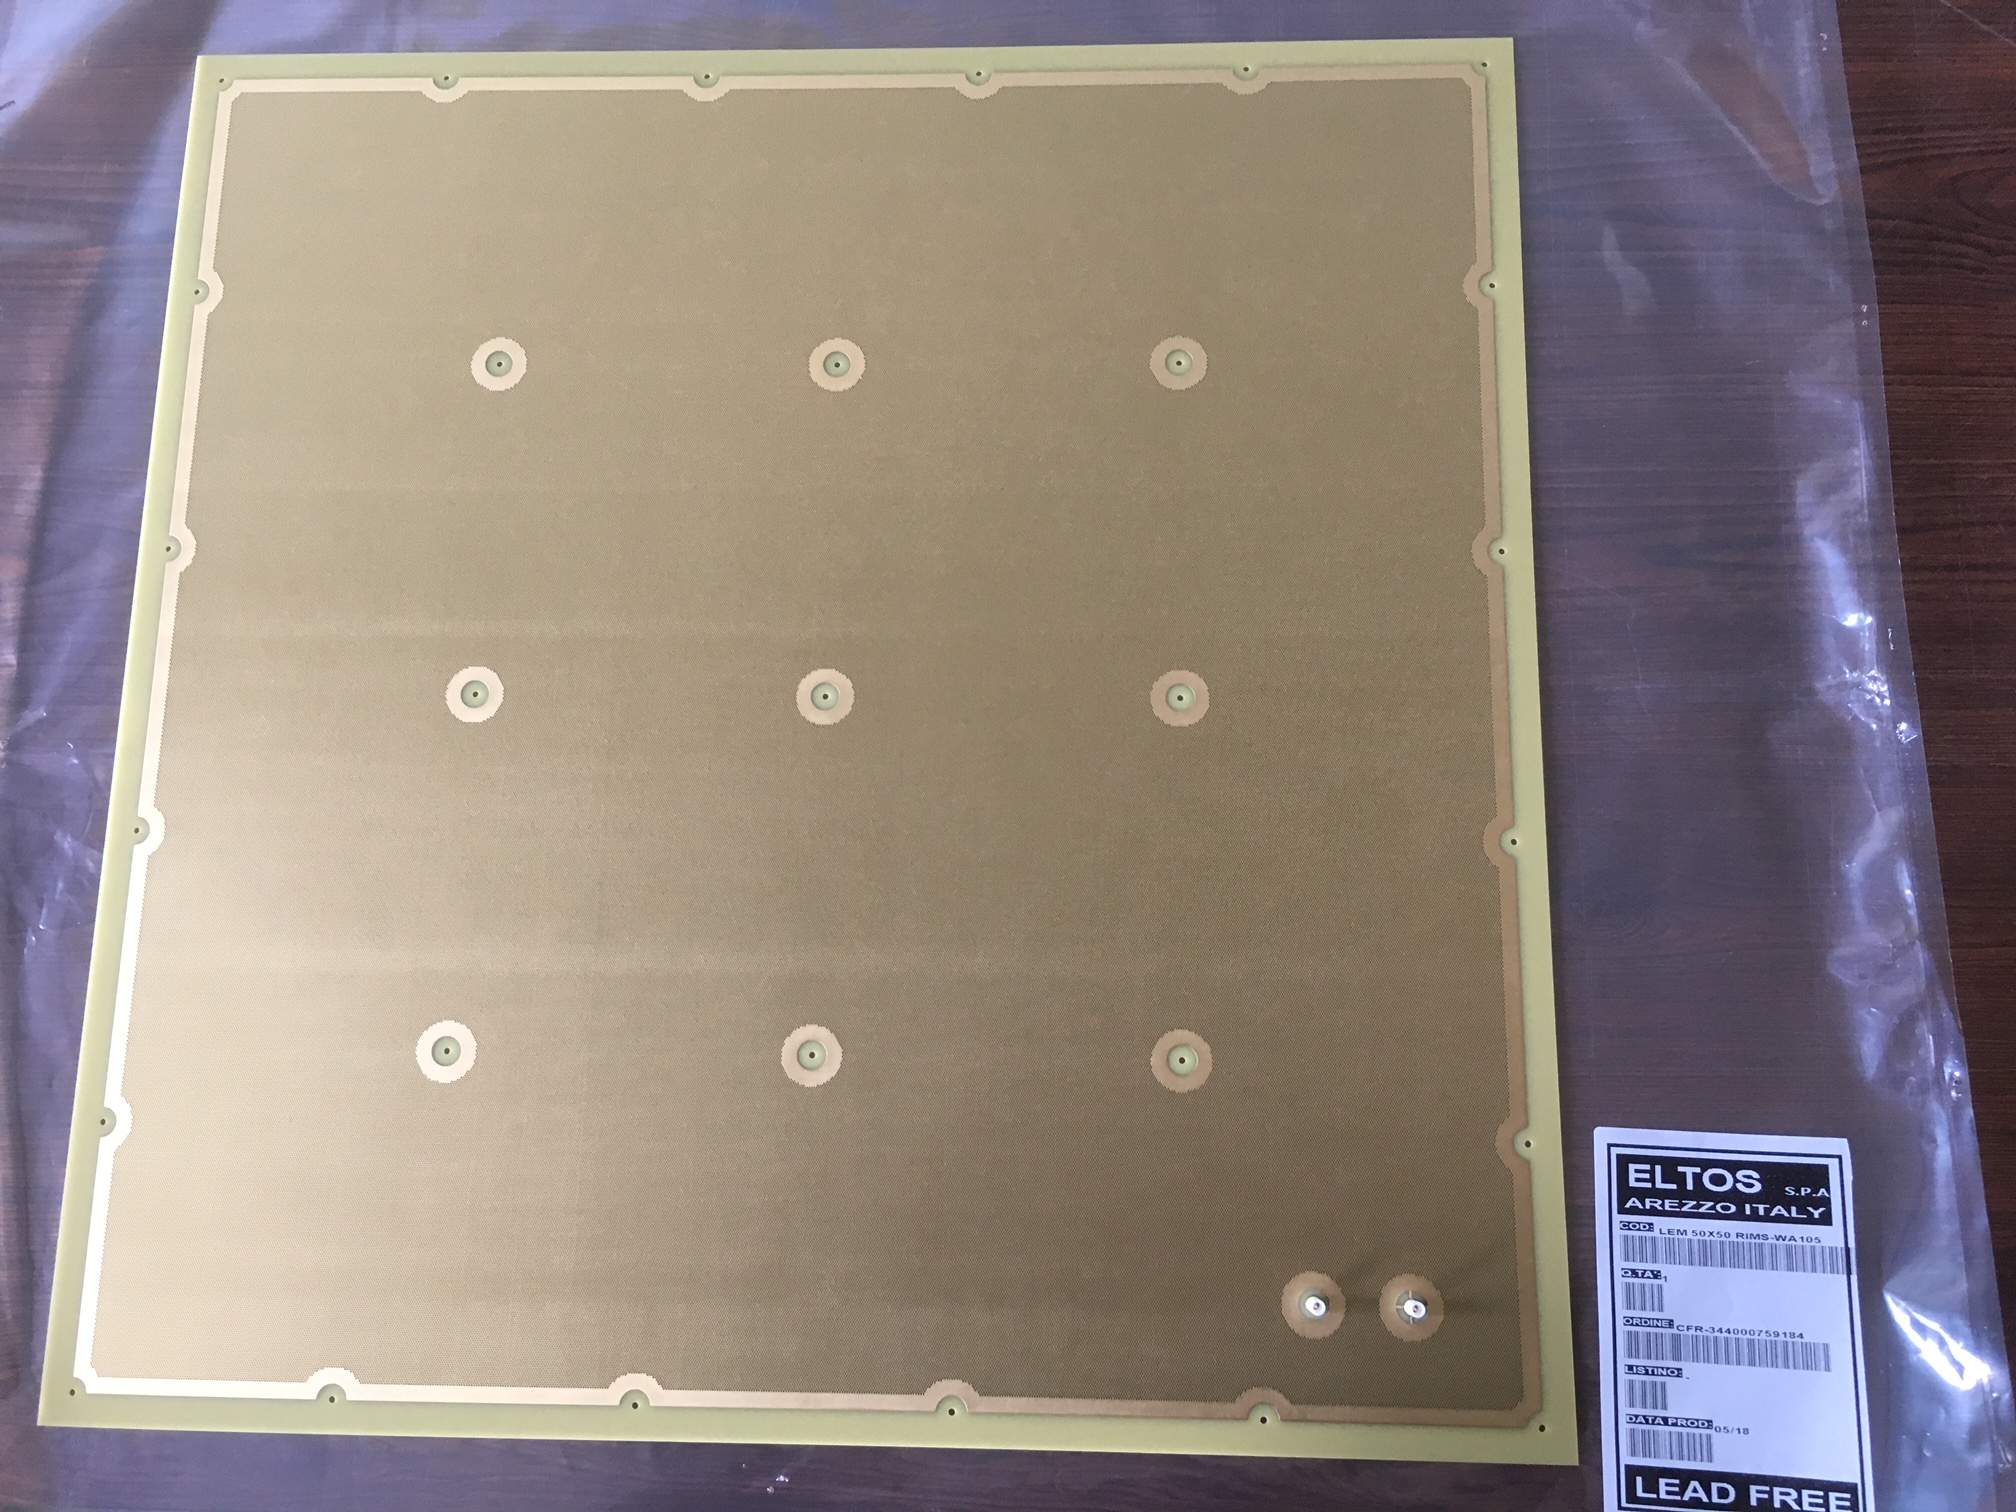
\includegraphics[width=.8\textwidth]{LEM_CFR-35.jpg}
\end{dunefigure}

%%%%%%%%%%%%%%%%%%%%%%%%%%%%%%%%%%%
\subsection{Anode}
\label{sec:fddp-crp-anode}
 
The anode is a four-layer PCB having a set of orthogonal strips with a \dpstrippitch pitch that provide the two views of the collected charge. The area of the anode is  \num{50}$\times$\SI{50}{cm$^2$}, identical to the \dword{lem} one. Twenty nine holes of \SI{2.2}{mm} diameter matching the \dword{lem} holes are used for the \dword{lem} and anode assembly on their G10 frame. The \SI{2}{mm} distance between the anode and the \dword{lem} is ensured by \num{29} precisely machined spacers made of polyetheretherketone (PEEK). 

The pattern of readout strips, printed on the bottom PCB layer and used for charge collection, is optimized such that the charge is evenly split between both views (Figure~\ref{fig:Anode}). Electrical insulation in the locations where orthogonal tracks would superimpose is achieved by 
%having tracks crossing over and under each other using a system of vias between the top and bottom layers of the PCB. 
using a system of vias between the top and bottom layers of the PCB to allow the tracks to cross over and under one another. 
Each strip, made of thin gold-plated copper tracks, has a capacitance per unit length to ground of about 
\SI{160}{pF/m}. The readout strips are routed to the top layer towards \num{68}-pin female connectors (KEL 8925E-068-179-F) soldered on the anode periphery. Each connector reads \num{32} strips; its \num{36} remaining pins are connected to the detector ground via a copper strip that runs around the periphery of the top layer of the anode (see Figure \ref{fig:Anode_CTest}). 

\begin{dunefigure}
[Picture of the anode symmetric \twod strip design.]
{fig:Anode}
{Picture of the anode symmetric \twod strip design.}
  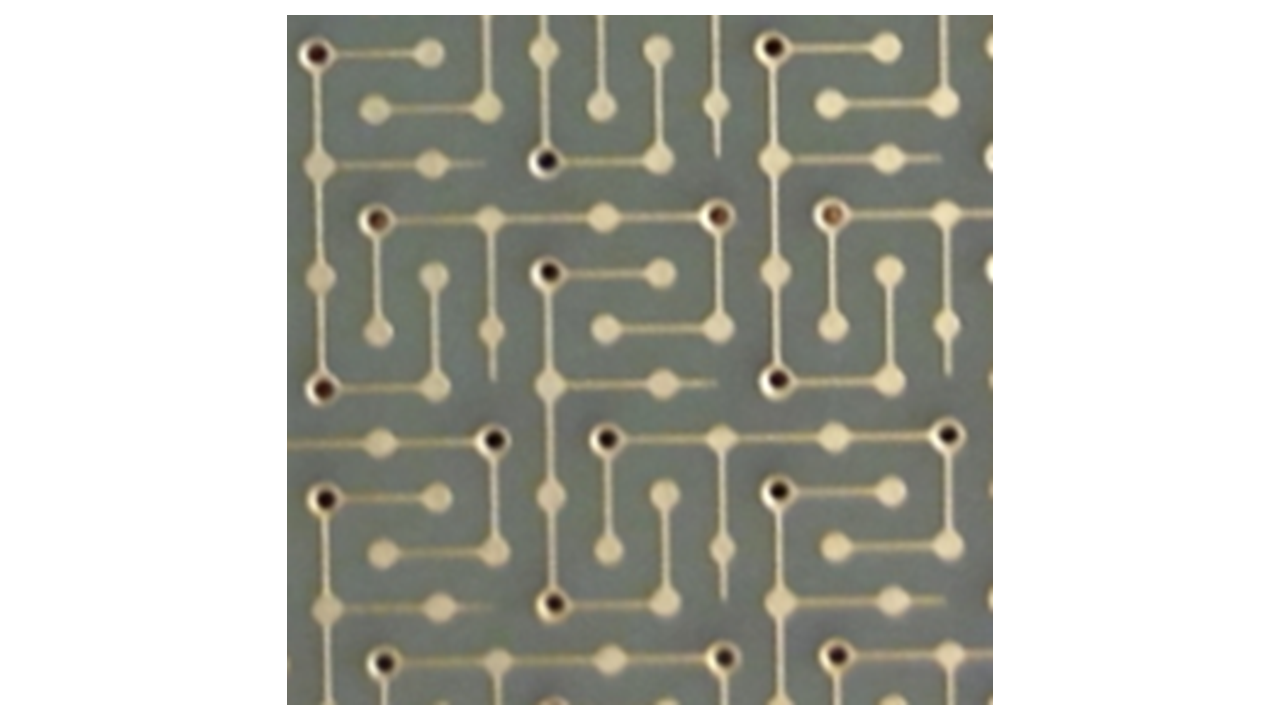
\includegraphics[width=.8\textwidth]{Anode_strips.png}
\end{dunefigure}

%%%%%%%%%%%%%%%%%%%%%%%%%%%%%%%%%%
\subsection{Instrumentation}
\label{sec:fddp-crp-instr}

\subsubsection{Distance meters and level meters}

The vertical and lateral positions of the \dwords{crp} are measured by different means. 
It is possible to know the vertical position of the \dword{crp} both from the suspension system and from dedicated capacitive measurements.
The  suspension system and its motorization on three points provides an accurate measurement for each \dword{crp} of order\SI{0.1}{mm} due to the accuracy of the steps motors and encoders. 
In order to exploit the information from the encoders,  the anchor points on the \dword{crp} must be surveyed during construction and the absolute positions of the suspensions must be surveyed from the roof of the cryostat during the installation of the \fdth.

There will be also the possibility to get relative measurements of the \dword{crp} position with respect to the \lar level using capacitive level meters put on the sides of the \dword{crp}s located at the periphery of the detection plane.  The  measurements of the capacitance between the \dword{lem} and the extraction grid, which depends on the height of the liquid above the grid, can also provide a relative measurement  of the \dword{crp}'s vertical position with respect to the liquid surface. This method is used for the \dword{crp}s which are not located at the periphery, while the ones at the periphery can exploit both the  \dword{lem}-grid capacitance measurements and the capacitive level meters.
 
% \fixme{prev pgraph needs work but I don't understand it well enough to improve it; some accuracy vs precision issues too} Rephrasing performed
 
The measurement of the distance between each \dword{crp} pair is performed by using capacitive devices called \textit{distance meters} made of two parallel plates. %will be used for 
This measurement enables positioning of the \dwords{crp} with the correct  inter-\dword{crp} distance all along the detection plane. These devices do not require any contact among  \dword{crp}s and give an accuracy of the order of \SI{0.1}{mm} on the  inter-\dword{crp} distance.  Four devices per \dword{crp} side are embedded in the G10 frame side as can be seen on Figure~\ref{fig:distancemeter}.

\begin{dunefigure}[View of the distance meter plates on the sides of a \dword{crp}]{fig:distancemeter}
{CAD views (left, center) of the distance meter plates, represented by the yellow rectangles, on the sides of a \dword{crp}. Two different plate sizes are used in pairs facing from one \dword{crp} to the neighbour one in order to increase the measurement accuracy of the overlapping surface which translates in the capacitance to be measured. A set of five distance meter plates of the two sizes (right) received from the production factory}
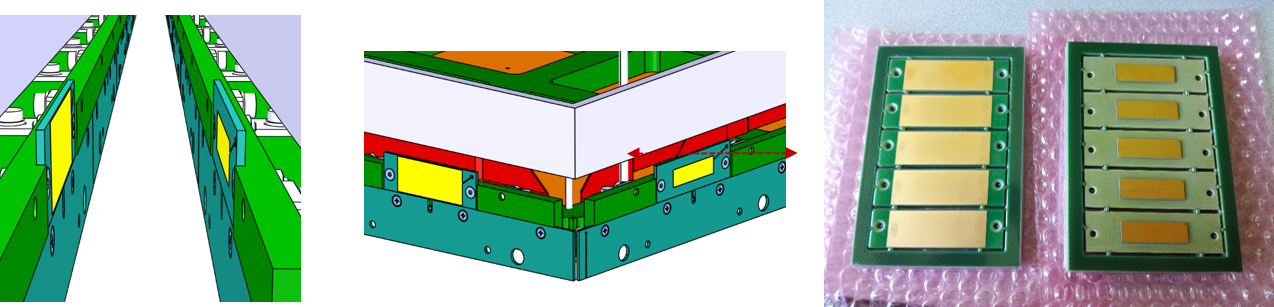
\includegraphics[width=0.85\textwidth]{distancemeter.png}
\end{dunefigure}

%\fixme{Fig \ref{fig:distance meter} could use more explanation} DONE

\subsubsection{Thermometers}

The temperature in the gas above the anode plane is monitored at different heights with resistance thermometers (Pt sensors) soldered on  six PCB boards distributed over the full surface of the \dword{crp}, six 
sensors per PCB. The configuration and the Pt positions are shown in Figure~\ref{fig:ptsensor}.

\begin{dunefigure}[View of the thermometer board]{fig:ptsensor}
{View of the thermometer board and the positions of the Pt sensors along the PCB plate.}
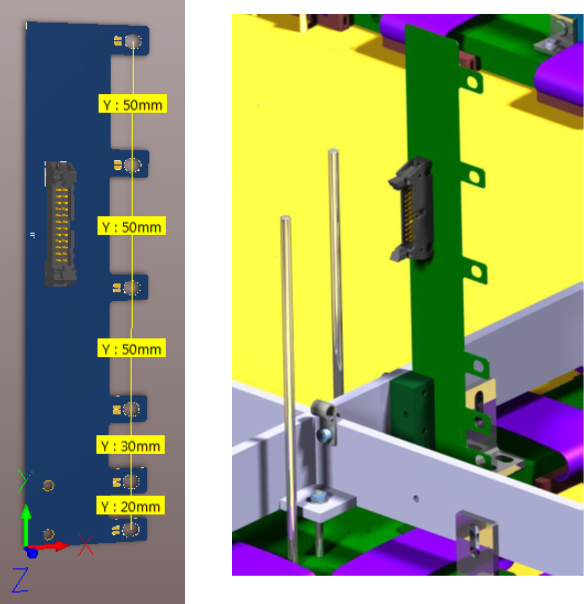
\includegraphics[width=0.35\textwidth]{ptsensor.png}
\end{dunefigure}

%%%%%%%%%%%%%%%%%%%%%%%%%%%%%%%%%%%
\subsection{Suspension System and Drive}
\label{sec:fddp-crp-suspension}

Three suspension \fdth{}s are arranged in an equilateral triangle whose barycenter coincides with that of the \dword{crp}; an automated system is used to suspend the \dword{crp} at the required position and precisely adjust the \dword{crp} level with respect to the \lar surface.

Figure~\ref{fig:spft} shows the design of the suspension \fdth including the bellows and the motors. There are three \fdth{}s per \dword{crp}.

\begin{dunefigure}[Suspension \fdth and various assembly details]{fig:spft}
{Suspension \fdth and various assembly details.}
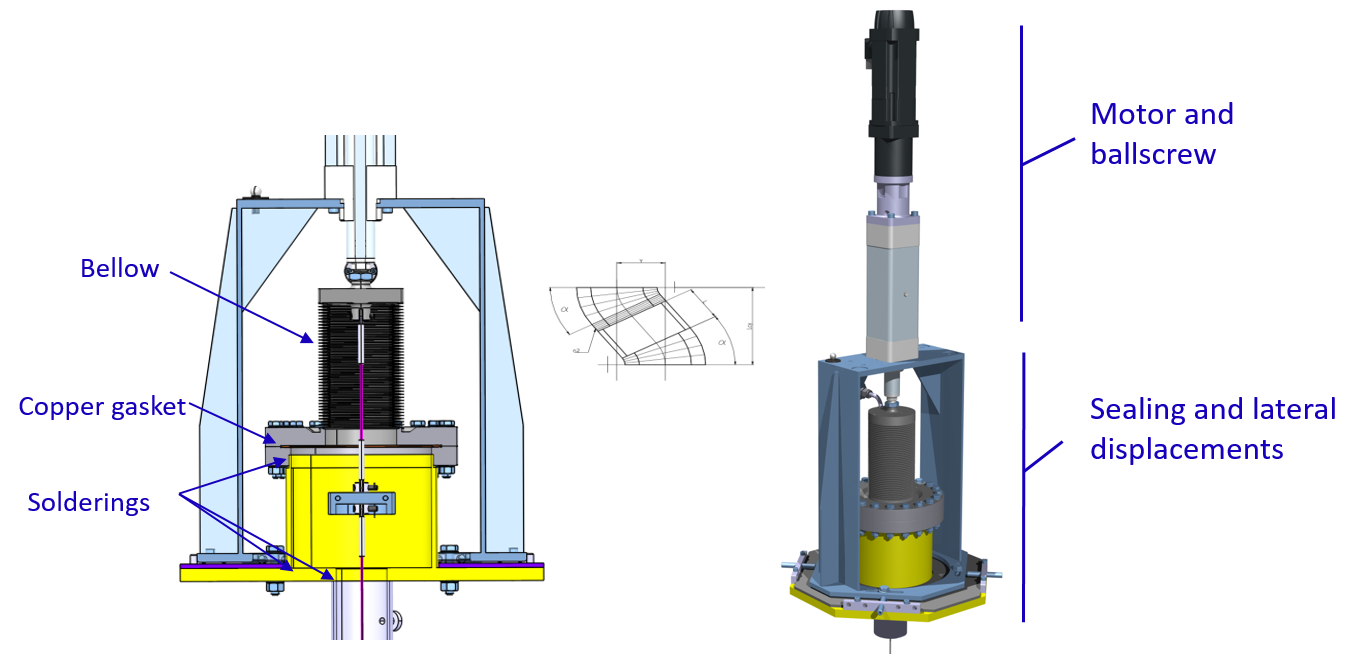
\includegraphics[width=0.7\textwidth]{spft.png}
\end{dunefigure}

At the level of the flanges on the crysotat roof the adjusting table on which the suspension \fdth is screwed allows a lateral stroke of \SI{26}{mm}. Any tranverse movement is absorbed by lateral deformation of the bellows.
The vertical stroke available with the bellows size is $\pm$\SI{20}{mm}.
The system incorporates a  mechanical stop and a simple obstruction of the chimney for maintenance purpose or bellows replacement.
At the top pf the suspension \fdth there is a special slot to position a laser tracker target
such that the \fdth position can be precisely surveyed during installation.

The suspension cables anchoring system on the \dword{crp} is shown in Figure~\ref{fig:anchor}. 
In case of variation of the cryostat pipes' verticality, this system allows to change an anchoring point on a module, in warm conditions. In cold conditions, the transverse movement is done with the suspension \fdth position adjustment.
\begin{dunefigure}[Anchoring system of the suspension cable on the \dword{crp} frame]{fig:anchor}
{Anchoring system of the suspension cable on the \dword{crp} frame.}
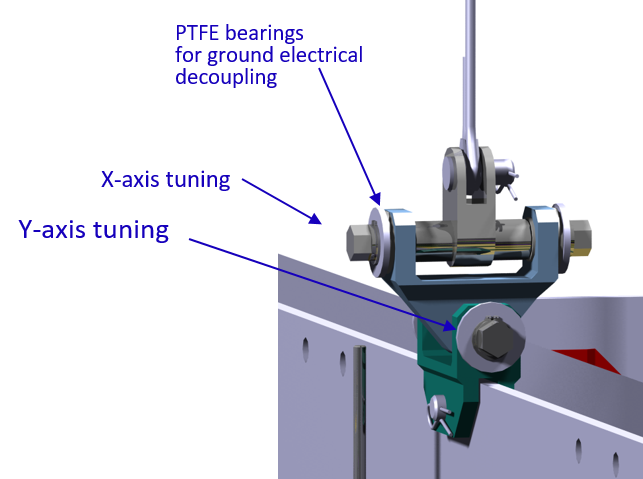
\includegraphics[width=0.6\textwidth]{anchor.png}
\end{dunefigure}

Each motor has independent controls for tuning the horizontality of the plane using the  level information output from the %different available 
sensors. In standard, stable running  conditions several \dword{crp} modules are associated together as a global system and controlled via an automatic process.

%\fixme{I don't understand this. what's a master ``axis''?} REMOVED

%%%%%%%%%%%%%%%%%%%%%%%%%%%%%%%%%%%
%\subsection{Quality Assurance}
%\label{sec:fddp-crp-qa}

%%%%%%%%%%%%%%%%%%%%%%%%%%%%%%%%%%%%%%%%%%%%%%%%%%%%%%%%%%%%%%%%%%%%
\section{Production and Assembly}
\label{sec:fddp-crp-prod-assy}

%%%%%%%%%%%%%%%%%%%%%%%%%%%%%%%%%%
\subsection{G10 and Invar Frame Production}
\label{sec:fddp-crp-frame}

% new from DD
The G10 and Invar frames are both produced by industry. For the \dword{dpmod}, %80
\dptotcrp Invar frames and \dpnumpmtch %720 
G10 subframes of \SI{1}{m$^2$} are required. %should be produced.
For \dword{pddp}, the process and \dword{qc} procedures have been defined.
For the Invar structure, SDMS\footnote{SDMS\texttrademark{}, \url{www.sdms.fr/en}.}, the company chosen for \dword{pddp}'s four \dwords{crp},  %managed the realization 
has produced them within the specifications without identified problems.
They had to organize the procurement of raw Invar plates, which depends on the available world stock. For the \dword{dpmod} it is important to plan ahead, %should be well anticipated
 for this procurement. 
% \fixme{I cannot find the url for SDMS (anne)} DONE
The manufacturing process followed by the manufacturer (SDMS) included eight steps:\\
\begin{itemize}
\item Plate rectification,
\item  Laser cutting,
\item  Assembly,
\item  Welding,
\item  Geometrical controls,
\item  Washing,
\item  Packing, and
\item  Shipping.
\end{itemize}

During the process a special validation step was included  for a full-size test frame to verify all the technical aspects and conformity to the requirements. 
The acceptance tests are performed on the geometry, the welding quality and the proper position of the different holes made in the Invar beams.

For \dword{pddp}, fabrication of the G10 frames for the four \dwords{crp} was done by a company with expertise in composite materials. The manufacturing process includes the %realization 
production of frames with fiber layers in different orientations as explained in Section~\ref{sec:invar-frame}, the drilling of more than \num{100} screw threads per square meter of G10 frames, among them \num{80} with a \SI{2}{mm} diameter.
The acceptance tests are mostly based on geometrical and dimension criteria, and quality of the threads.  
The G10 production is longer and more difficult than that for the Invar structure. G10 production would require a minimum of two production sites, while one company would suffice for the Invar frame production.
%%% end new from DD


%%%%%%%%%%%%%%%%%%%%%%%%%%%%%%%%%%
\subsection{LEM and Anode Production}
\label{sec:fddp-crp-LASprod}


The construction of a  %10\,kT far detector based on the Dual Phase \lar technology
\dword{dpmod} involves the production of \dpnumswch charge readout modules made of a \dword{lem} and its anode. For such a large production, it is desirable to use more than one manufacturer in order to mitigate risks and costs. The ELTOS\footnote{ ELTOS\texttrademark{} \url{www.eltos.com}.} company in Italy is making the \dword{lem} modules and the anodes for  \dword{pddp} and as such, has successfully worked out the \dword{qa} and \dword{qc} processes based on requirements and specifications agreed with the \dword{wa105} collaboration. So far, the fraction of rejected \dword{lem} modules produced by ELTOS, after the final phase of tests, has proven to be small, less than one \dword{lem} per \dword{crp}. The rejection factor for the anodes is, however, higher and corresponds to about \SI{10}{\%}, due to the very thin and fragile conducting strips forming the anode plane and also to the close proximity of the outer strips to the PCB edges. 

%\fixme{``...to the close proximity of these strips to the PCB edges''?} DONE

Small modifications to the anode design will be necessary for the \dword{dpmod} in order to increase the robustness of the manufacturing process. It is believed that such modifications are possible without  %can be envisaged without affecting 
significantly affecting the performance of the anode.   

A second manufacturer, ELVIA\footnote{ELVIA\texttrademark{} \url{https://www.pcb-elvia.com/}.} in France, is also known to have the capability for large-scale \dword{lem} and anode production with the requested specifications. Recently, several \dword{lem} prototypes have indeed been built for CEA/Irfu 
%\fixme{lrfu?} Irfu is an institute of CEA
by ELVIA and extensive tests have %shown %that the same \dword{lem} performance as with ELTOS could be achieved.
demonstrated the same  \dword{lem} performance as the ELTOS products achieve.
 One key issue for a very large production, like the one necessary for DUNE, is to establish thorough \dword{qa} and \dword{qc} processes that can be applied throughout the whole \dword{lem} production. The definition of the \dword{lem} manufacturing requirements and specifications is naturally an important part of the tendering process. As far as the anodes are concerned, several prototypes have already been manufactured by ELVIA with satisfactory results. Despite the large size (\num{50}$\times$\SI{50}{cm$^2$}) of the anode, its fabrication follows a rather standard process mastered by several PCB manufacturers in Europe and around the world.     

%%%%%%%%%%%%%%%%%%%%%%%%%%%%%%%%%%
\subsubsection{LEM production and QA and QC}
\label{sec:fddp-crp-LEMprod}

In the following scheme, an effective production time of \num{40} weeks per year and a total duration of two years is assumed. This corresponds to an average \dword{lem} production rate of one \dword{crp} or \num{36} \dword{lem} modules per effective week. The main limitation to the manufacturing speed comes from the \dword{lem} drilling process. While it is likely that ELTOS and ELVIA will have the capability each to produce \num{18}  \dword{lem} modules per week by assigning dedicated drilling machines, it would still be highly advisable to identify, well before the start of the \dword{lem} production phase, additional manufacturers capable of large-scale production. 

Based on the experience gained with  \dword{pddp}, the  \dword{qa} and \dword{qc} requirements during the \dword{lem} manufacturing process include the selection of the base material for the \dword{lem} PCB, thickness measurements of the dielectric material and copper layers before and after the process, a control of the size of the \dword{lem} holes, rims and outer dimensions, as 
well as a measurement of the electrical insulation across the two faces of the PCB.  
Table~\ref{tab:LEM_Tolerance} gives, as an example, the requested tolerance values on the various parameters of the \dword{lem} detectors for  \dword{pddp}. In addition, pre-series productions of several \dword{lem} modules from each manufacturing site will be necessary in order to validate the complete fabrication process prior to the start of the full production.

\begin{dunetable}[Tolerance values on various \dword{lem} parameters]
{p{.4\textwidth}p{.30\textwidth}}
{tab:LEM_Tolerance}
{Tolerance values on various \dword{lem} parameters} 
Parameter & Value and tolerance \\ \toprowrule
%  & \\ 
Dielectric thickness & \num{1.00}$^{+0.00}_{-0.05}$\,mm \\ \colhline
%  & \\ 
Average total thickness & \num{1.20}$^{+0.00}_{-0.06}$\,mm \\ \colhline
%  & \\ 
Dimensions & \num{499.5}$^{+0.00}_{-0.30}$\,mm$\times$499.5$^{+0.00}_{-0.30}$\,mm \\ \colhline
%  & \\ 
Final PCB thickness & \num{1.10}$^{+0.02}_{-0.05}$\,mm \\ \colhline
%  & \\ 
Active hole diameter & \num{0.50}$^{+0.00}_{-0.01}$\,mm \\ \colhline
%  & \\ 
Rim size & \num{40}$\pm$4\,$\mu$m \\ \colhline
%  & \\   
Electrical insulation & >\SI{1}{\giga\ohm} \\
 \end{dunetable}

Once manufactured, the \dword{lem} modules are shipped to one or several collaboration sites for their final characterization and validation. Several infrastructures are necessary in order to performthese tasks, e.g., a survey bench, clean rooms and storage rooms, cleaning stations and \dword{hv} test setups. Here is a list of tasks to be performed, in sequential order:

\begin{itemize}
\item {\bf Visual inspection and survey.} Upon receipt of the \dword{lem} modules from the manufacturing sites, the first operations to be carried out are the visual inspection to examine the quality of the \dword{lem} surfaces, %and then,
followed by the detector survey. The parameters that determine the \dword{lem} amplification gain are the thickness of the PCB and the geometry of the holes. It is therefore important to assess the uniformity of these parameters over the entire area of a \dword{lem} module. For  \dword{pddp}, this is performed on a sampling basis with the use of a confocal laser scanning microscope (CLSM). Several hundred measurements are done in each of \num{25} predefined locations, distributed uniformly over the \dword{lem} surface. With such an optical system, the total \dword{lem} and copper layer thicknesses as well as the rim size can be measured with a precision of a few microns. For a very large production as for a \dword{dpmod}, the development of a fully automated survey system is mandatory. 

\item {\bf \dword{hv} connection.} The next step consists of soldering the \dword{hv} connection pins on the two \dword{lem} copper surfaces as well as gluing the MACOR insulators around the connectors.

\item {\bf Cleaning and polymerization.} The cleaning operation is an important phase of the \dword{lem} preparation. Following a procedure defined by CERN/EP-DT-EF-MP and CEA/Irfu,
%\fixme{should these be references?} we do not have at  the moment a written document which can be referred to
 this is done using an ultrasonic bath at \SI{65}{C} with a micro-finishing solution (NGL 17.40 Sp ALU III) to clean the gold-plated copper surfaces of the \dword{lem}. It is followed by a rinsing phase with water and then with a spray of pressurized deionized water %sprayed under pressure 
 ($<$\,30\,bar). The \dword{lem} is then dried in an oven 
at \SI{60}{C}  for several hours and then baked for three hours up to \SI{160}{C}, %at 
a temperature near the glass transition point of the dielectric material. From the cleaning operation on, each \dword{lem} is handled via an aluminum frame on which it is mounted in order to avoid any contact with the PCB surfaces. They are also to be %Once cleaned, all \dword{lem} modules need in addition to be 
handled and operated in a clean environment with the use, for example, of a laminar flux.  

\item {\bf \dword{hv} tests.} The final validation of a \dword{lem} is obtained after  successful and stable operation in pure argon at room temperature and an absolute pressure of about \numrange{3.2}{3.3}\,bar. A high-pressure vessel is used for this purpose.  The argon pressure value is precisely adjusted as a function of the argon temperature inside the vessel in order to reach the same gas density as the one existing in D\lar mode. In such a way, the \dword{lem} modules are tested at the same Townsend avalanche operation point as in cold. Figure~\ref{fig:HP} shows the \SI{360}{L} high-pressure vessel used at CEA/Irfu for the characterization of the  \dword{pddp} \dword{lem} modules. Up to nine \dword{lem} modules can be stacked inside this chamber for the \dword{hv} tests. The HP vessel is also instrumented with \dword{fe} electronics and a \dword{daq} system for gain measurements in pure argon. In this configuration, a single \dword{lem} is installed with its \twod charge-collecting anode inside 
a \num{50}$\times$\num{50}$\times$\SI{5}{cm$^3$} 
TPC together with a collimated $^{241}$Am open alpha source mounted on 
the cathode. Figure~\ref{fig:HP_ED} shows an event display of a \SI{5.5}{MeV} alpha track observed in pure argon gas at an 
absolute pressure of \num{1}\,bar.
%
During the \dword{lem} validation \dword{hv} tests, a two-step procedure is followed. After pumping for 
about \num{60} hours down to a residual pressure of \num{10}$^{-4}$\,mbar, the chamber is filled with dry synthetic air and 
\dword{hv}  up to \SI{4.5}{kV} is applied across the \dword{lem} in order to 
burn possible residual dust. Then, the vessel is pumped again and pure argon (graded \num{5.7})
is introduced at an absolute pressure of about \numrange{3.2}{3.3}\,bar. Each \dword{lem} module is tested 
and validated so see that it can reach the value of \SI{3.5}{kV} across the two faces, consistent with amplification gains higher than \num{100} before charging up, with no occurrence of discharges. The amount of time needed to perform the \dword{hv}  tests is 
typically one week for an entire batch of nine \dword{lem} modules. This last figure can probably be increased to \num{12} with a slightly larger volume vessel. 
\end{itemize}

While the tasks related to the \dword{lem} visual inspection, survey and the implementation of the \dword{hv}  connections can be done at 
a single participating institution %collaboration 
site, the subsequent operations could be dispatched among several sites. In that case, it is  important that each %Collaboration 
site %involved in the final validation steps 
have the necessary infrastructure for 
both the cleaning phase and the \dword{hv} tests, as iterations are sometimes necessary in order to fully validate the 
\dword{lem} modules. With the assumption of \num{36} \dword{lem} modules produced per effective week, a reasonable number of setups needed for the \dword{hv}  tests, together with their associated instrumentation and infrastructure, could amount to three or four. Finally, based on the experience gained in  \dword{pddp}, the processing time needed for the preparation, characterization and tests of a batch of nine to \num{12} \dword{lem} modules can be estimated to about three weeks.  

\begin{dunefigure}
[High-pressure vessel for the characterization of the  \dword{pddp} \dword{lem} modules.]
{fig:HP} 
{High-pressure vessel for the characterization of the  \dword{pddp} \dword{lem} modules.}
  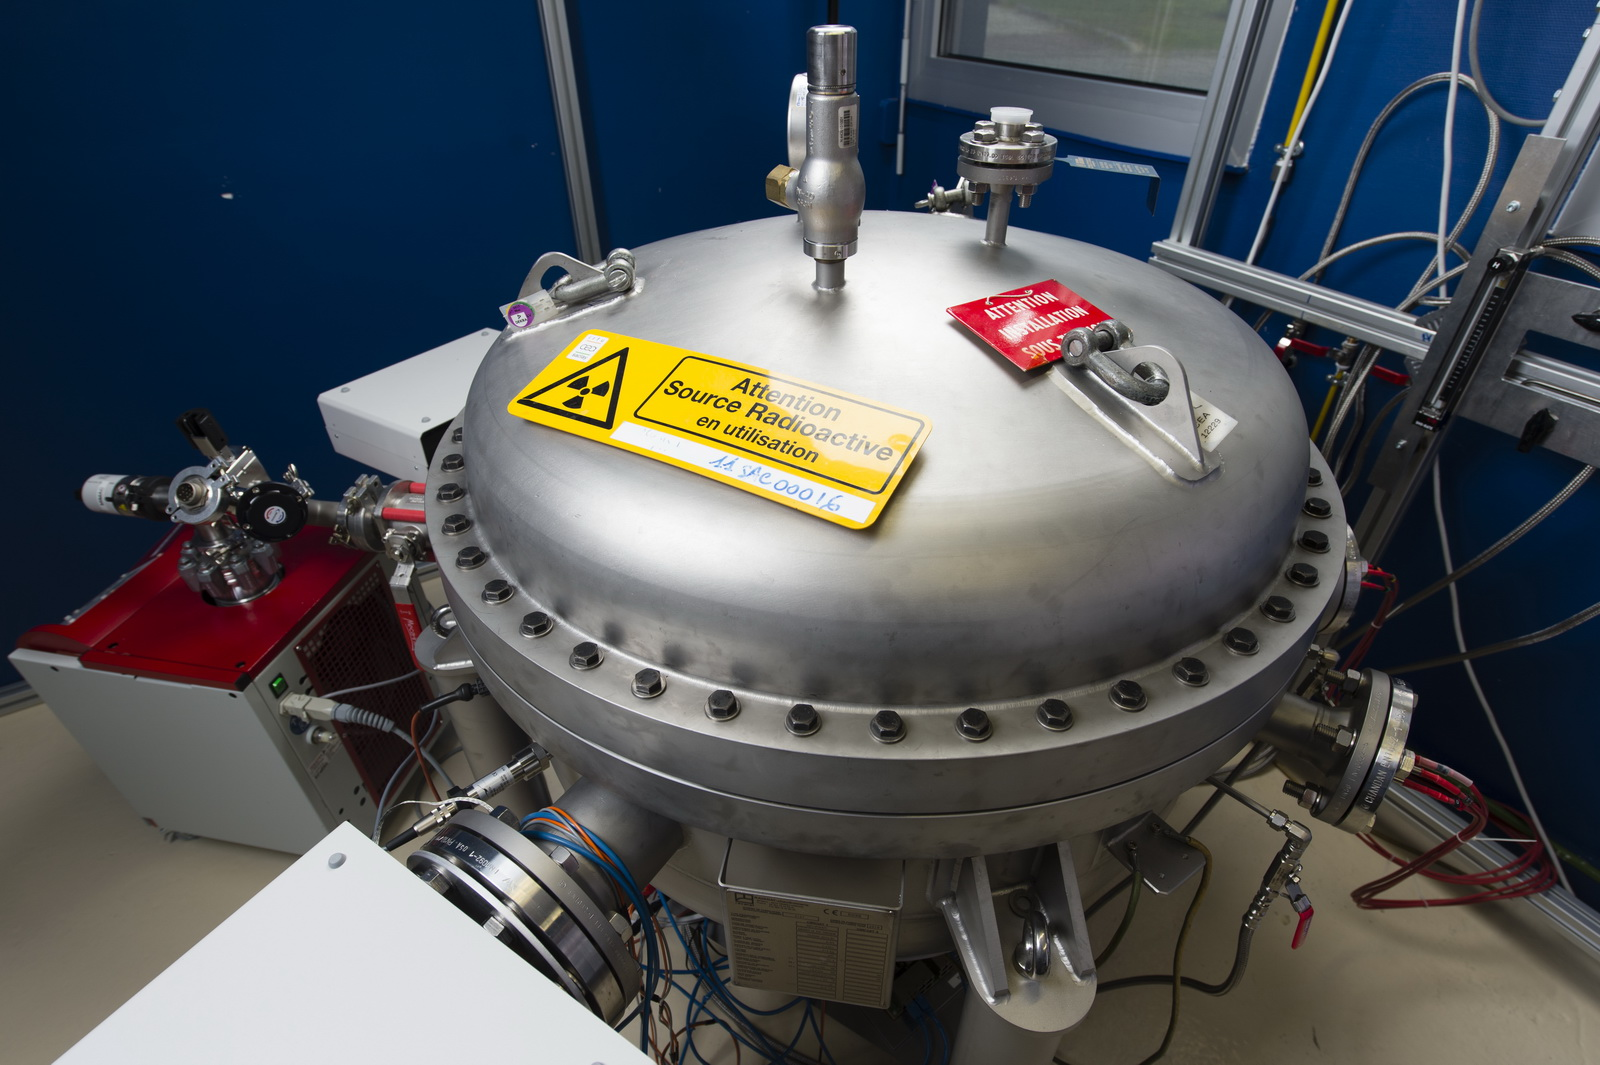
\includegraphics[width=.8\textwidth]{HP.jpg}
\end{dunefigure}


\begin{dunefigure}
[Event display of a \SI{5.5}{MeV} alpha track in argon gas at \num{1}\,bar.]
{fig:HP_ED}
{Event display of a \SI{5.5}{MeV} alpha track in argon gas at \num{1}\,bar.  Left: $x$-View. Right: $y$-View. Top: Pulse-height distributions of hits in \dword{adc} counts. Bottom: Hit time [300\,ns bins] -vs- strip number.}
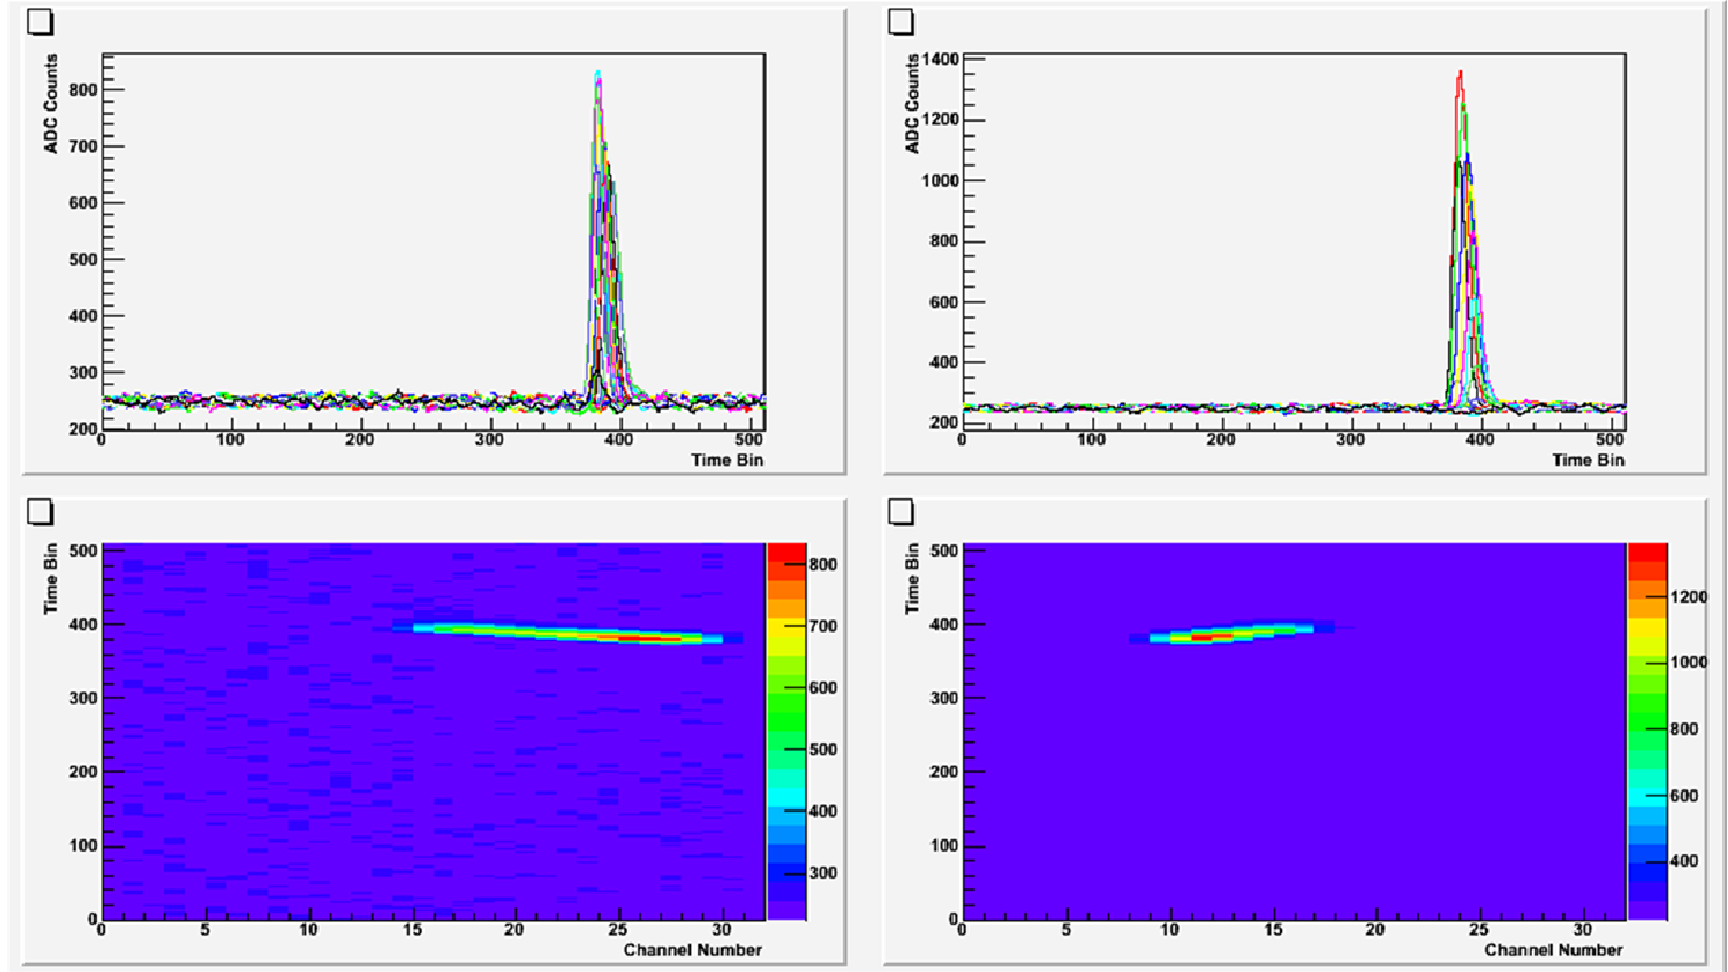
\includegraphics[width=.8\textwidth]{HP_ED.png}
\end{dunefigure}

%%%%%%%%%%%%%%%%%%%%%%%%%%%%%%%%%%
\subsubsection{Anode production and QA/QC}
\label{sec:fddp-crp-ANODEprod}
It is realistic to assume that the lead time in the manufacturing of the anodes will be compatible with the production time
of the \dword{lem} modules. Table~\ref{tab:ANODE_Tolerance} gives the anode specifications for the dimensions of the PCB. In addition, visual inspection and continuity tests are requested at the manufacturing site after the soldering of the signal connectors. Upon receipt at the collaborating institution site(s) where the \dword{crp} assembly will take place, continuity and short circuit tests of the anode strips are performed (see Figure \ref{fig:Anode_CTest}). This task is rather quick and should not take more than one day per \dword{crp}.  


\begin{dunetable}[Specifications for the anode dimensions]
{p{.4\textwidth}p{.30\textwidth}}
{tab:ANODE_Tolerance}
{Specifications for the anode dimensions} 
 Parameter & Value and tolerance\\ \toprowrule
%  & \\ 
Dimensions & 499.5$^{+0.2}_{-0.0}$\,mm$\times$499.5$^{+0.2}_{-0.0}$\,mm \\ \colhline
%  & \\ 
PCB thickness & 3.5$\pm$0.05\,mm \\ \colhline
%  & \\ 
PCB sagitta & < 1\,mm \\
 \end{dunetable}

\begin{dunefigure}
[Test of anode strip continuity]
{fig:Anode_CTest} 
{Test of anode strip continuity.}
 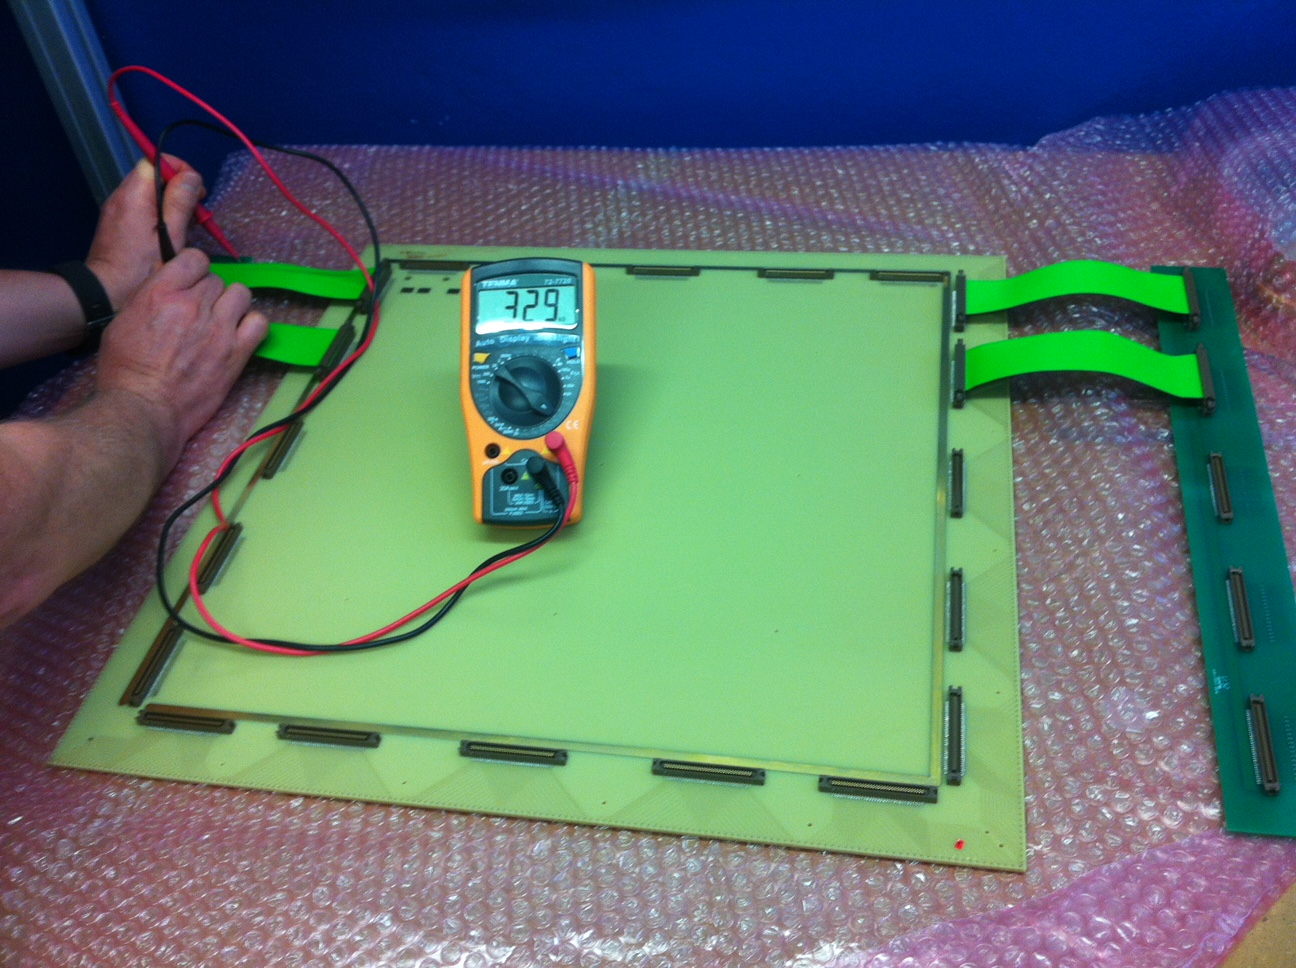
\includegraphics[width=.8\textwidth]{Anode_CTest.jpg}
\end{dunefigure}

%%%%%%%%%%%%%%%%%%%%%%%%%%%%%%%%%%
\subsection{Tooling}
\label{sec:fddp-crp-tooling}

%%% new from DD
Once the anodes, the \dwords{lem}, the mechanical Invar and G10 frames are produced and delivered, the \dwords{crp} production site should be equipped with several toolings.
The \dwords{crp} construction activity requires a clean room large enough to accommodate the different work spaces. Separate work areas are required in this clean room for: %It can be divided into four main work areas, requiring:
\begin{itemize}
\item{a \SI{10}{m$^2$} table for assembling the G10 subframes and for surveying the whole structure}
\item{a supporting structure to hang the Invar frame and to allow coupling of the G10 frame and the installation of the anodes, \dword{lem} and extraction grid modules.}
\item{storage of the anodes and \dwords{lem} on special shelves }
\item{construction of the extraction grid modules and storage of the modules before mounting on the \dword{crp} structure}
\end{itemize}
The required tooling includes: two mobile cranes (\SI{4}{m} span) to manipulate the Invar frame, an aluminum support frame and parts of the transport boxes, a large assembly table, storage shelves for the \dword{lem} and anodes and for cables, and a fabrication bench for the extraction grid modules.
Figure~\ref{fig:gridtooling} shows the \SI{3}{m} long wiring bench with details and the real tooling at CERN used for the \dword{crp} of \dword{pddp}.

\begin{dunefigure}[Extraction grid construction bench details]{fig:gridtooling}
{Extraction grid construction bench details and picture in the clean room 185 at CERN.}
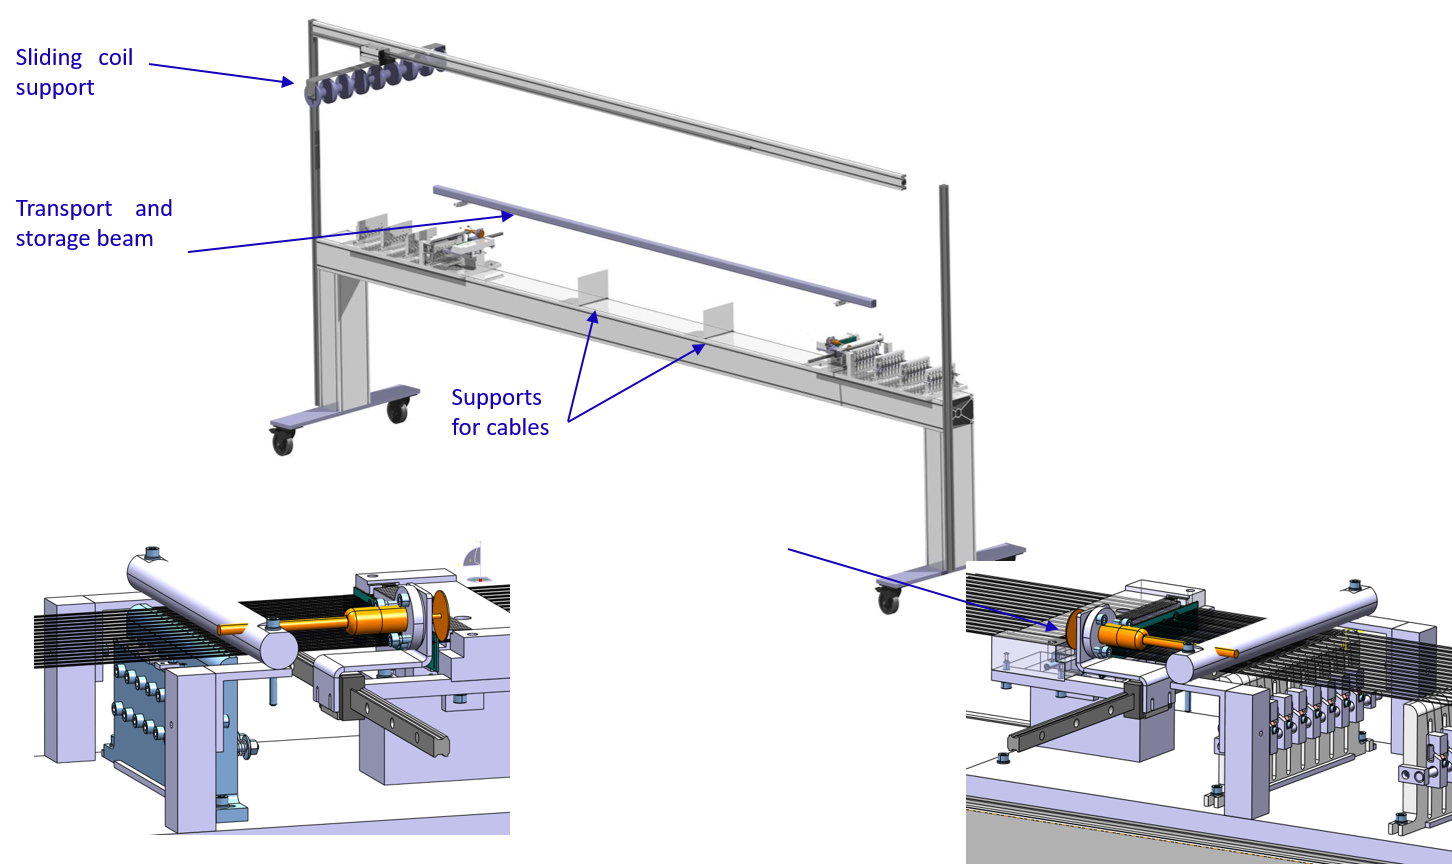
\includegraphics[width=0.65\textwidth]{grid-toolingv2.png}
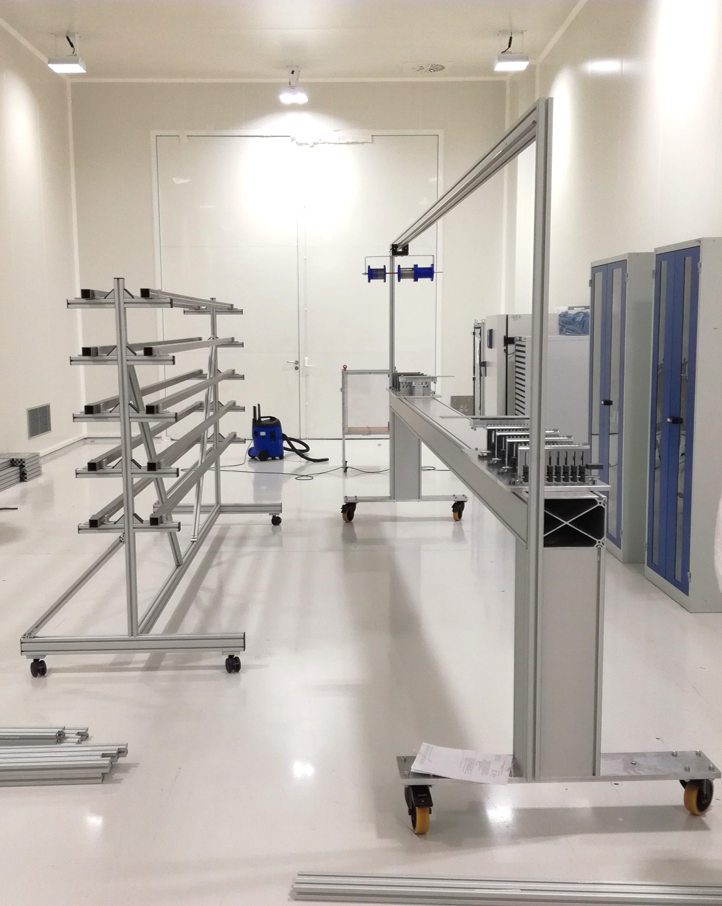
\includegraphics[width=0.3\textwidth]{grid-tooling185.png}
\end{dunefigure}
%%% end new from DD

%%%%%%%%%%%%%%%%%%%%%%%%%%%%%%%%%
\subsection{Assembly Procedures}
\label{sec:fddp-crp-assy}

The \dword{crp} assembly production activity will span two years 
%\fixme{span 2 yrs or > 2yrs?} 
prior to \dword{crp} installation underground at \surf. The \dwords{crp} will be integrated in at least two different production sites and stored locally in temporary storage boxes before being shipped to the \dword{itf}. % delivery facility. 
The \dword{crp} assembly will be pipelined with the \dword{lem} and anode production and testing during these two production years with an initial  shift of three months. This is intended to constitute a large enough buffer between the \dwords{lem} and anodes to start the \dword{crp} assembly activities.

%%% new from DD
The assembly of a \dword{crp} in the clean room is a process that goes from the reception of the Invar frame to the  closing of the transport box. 
A detailed animation of the assembly steps and procedures for the construction of a \dword{pddp} \dword{crp} is available\footnote{\url{https://www.youtube.com/watch?v=jcnJjlU-Cyc&feature=youtu.be}.}.
%The illustration of the assembly steps and procedures performed for the \dword{crp}  construction in the clean room in Building 185 at CERN for \dword{pddp} can be seen at \url{https://youtu.be/jcnJjlU-Cyc}.

This is divided in the following way:
\begin{enumerate}
\item Reception of the Invar frame in the clean room;
\item  Suspension of the Invar frame below the supporting structure;
\item  Vertical position of the frame is adjusted using lifting cranks;
\item  In parallel, assembly of the G10 frame proceeds on the optical table;
\item  The Invar frame is brought above the G10 frame, and connected through \num{50} decoupling systems;
\item  Assembly of \dword{lem} and anodes is done from below;
\item  Anodes are connected with jumpers;
\item  In parallel, the extraction grid is woven and soldered on the special tooling, then stored on shelves, or directly installed on the \dword{crp}.
\end{enumerate}
Some of the steps are illustrated in Figure~\ref{fig:assembly} and real components and tooling for \dword{pddp} are shown in Figure~\ref{fig:assembly2}.

\begin{dunefigure}[\dword{lem} and anode connection and extraction grid module installation.]{fig:assembly}
{Some assembly steps: \dword{lem} and anode connection and extraction grid module installation.}
%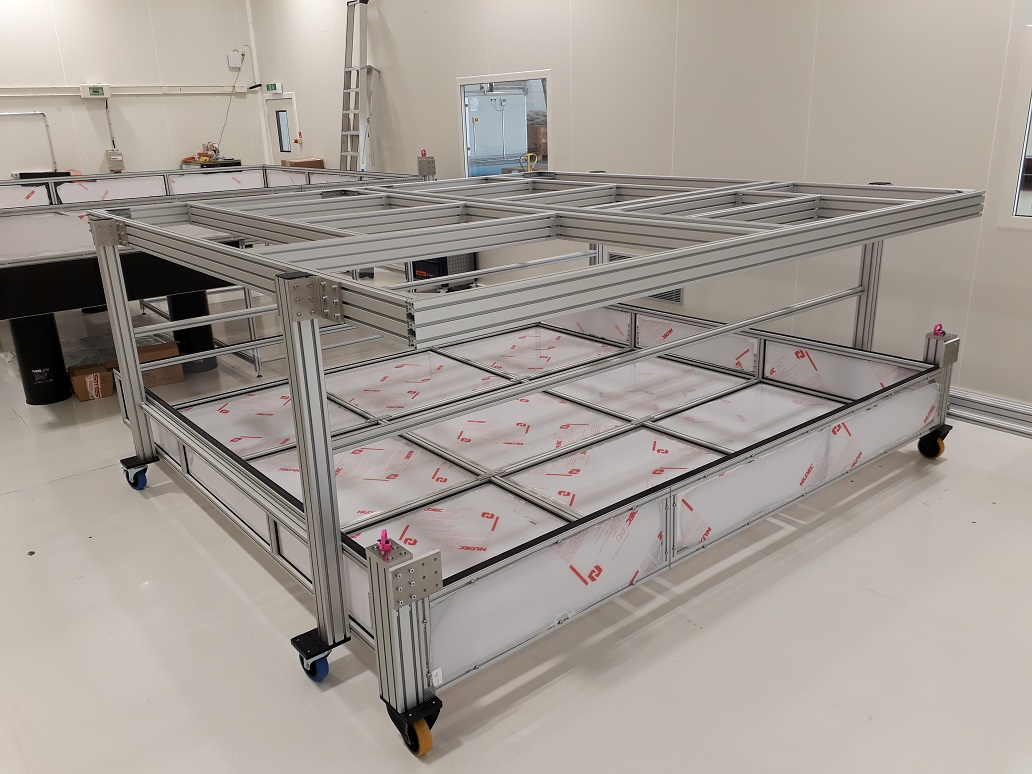
\includegraphics[width=0.25\textwidth]{structure-assembly.jpg}
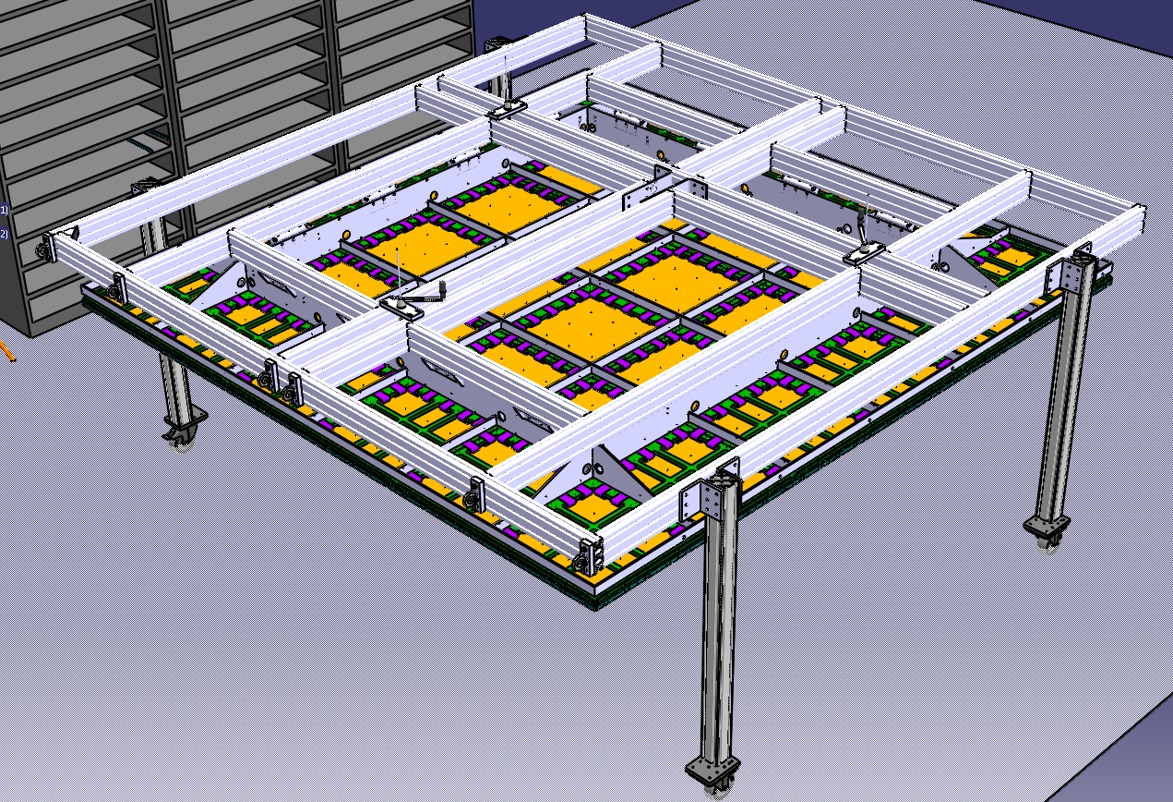
\includegraphics[width=0.3\textwidth]{assembly1.jpg}
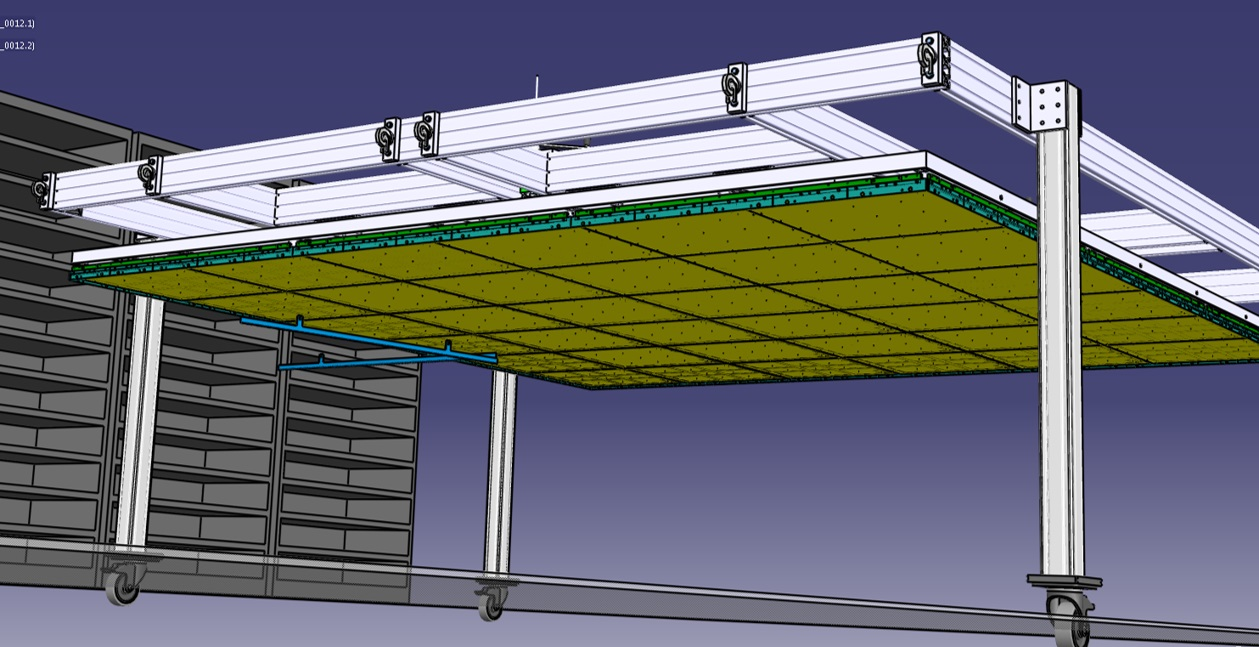
\includegraphics[width=0.35\textwidth]{assembly2.jpg}
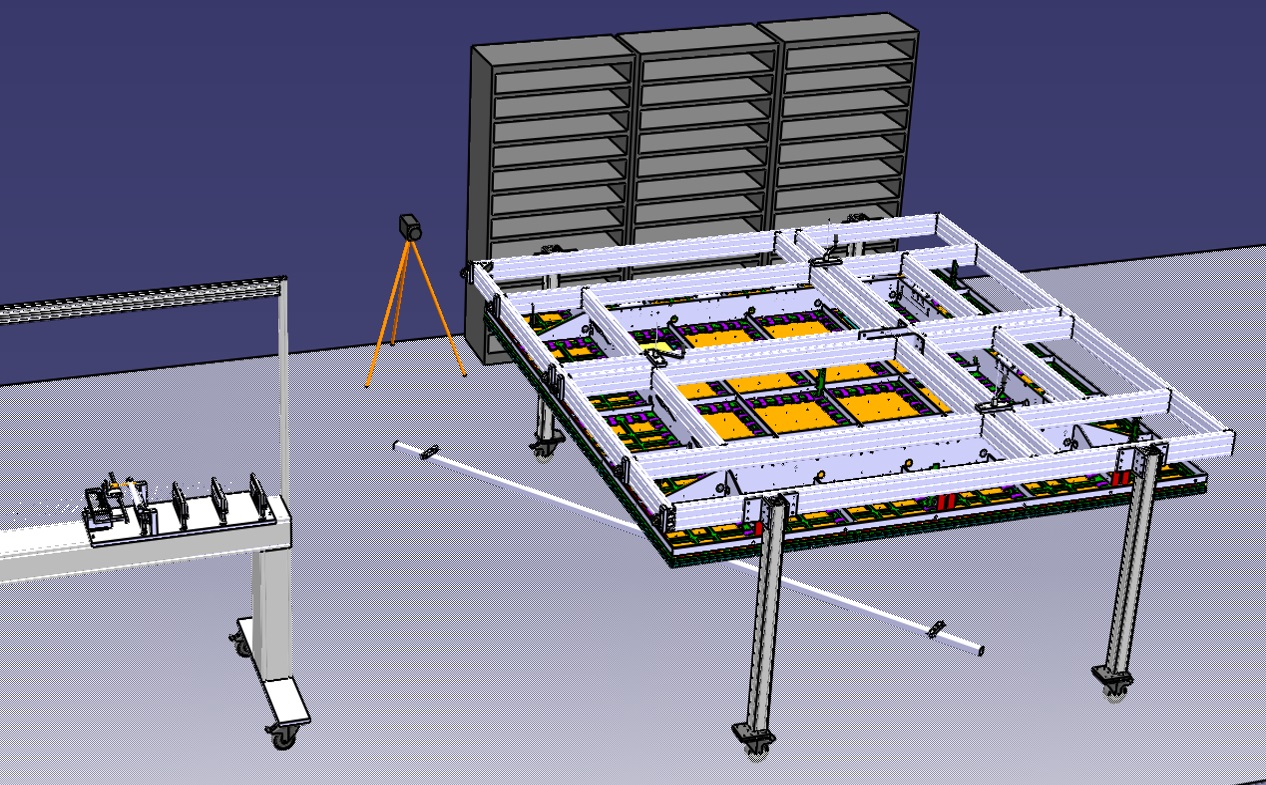
\includegraphics[width=0.3\textwidth]{assembly3.jpg}
\end{dunefigure}

\begin{dunefigure}[Elements for assembly of \dword{pddp} \dword{crp} at CERN]{fig:assembly2}
{Elements for assembly of \dword{pddp} \dword{crp} in clean room 185 at CERN: assembly structure and G10 subframes being prepared.}
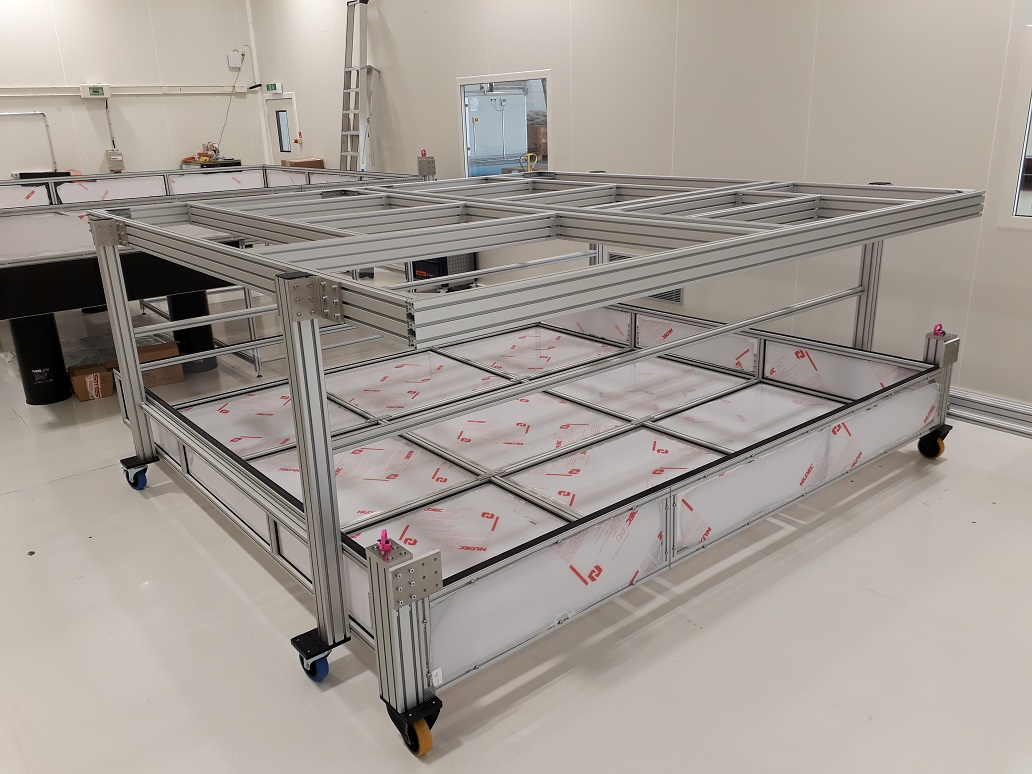
\includegraphics[width=0.4\textwidth]{structure-assembly.jpg}
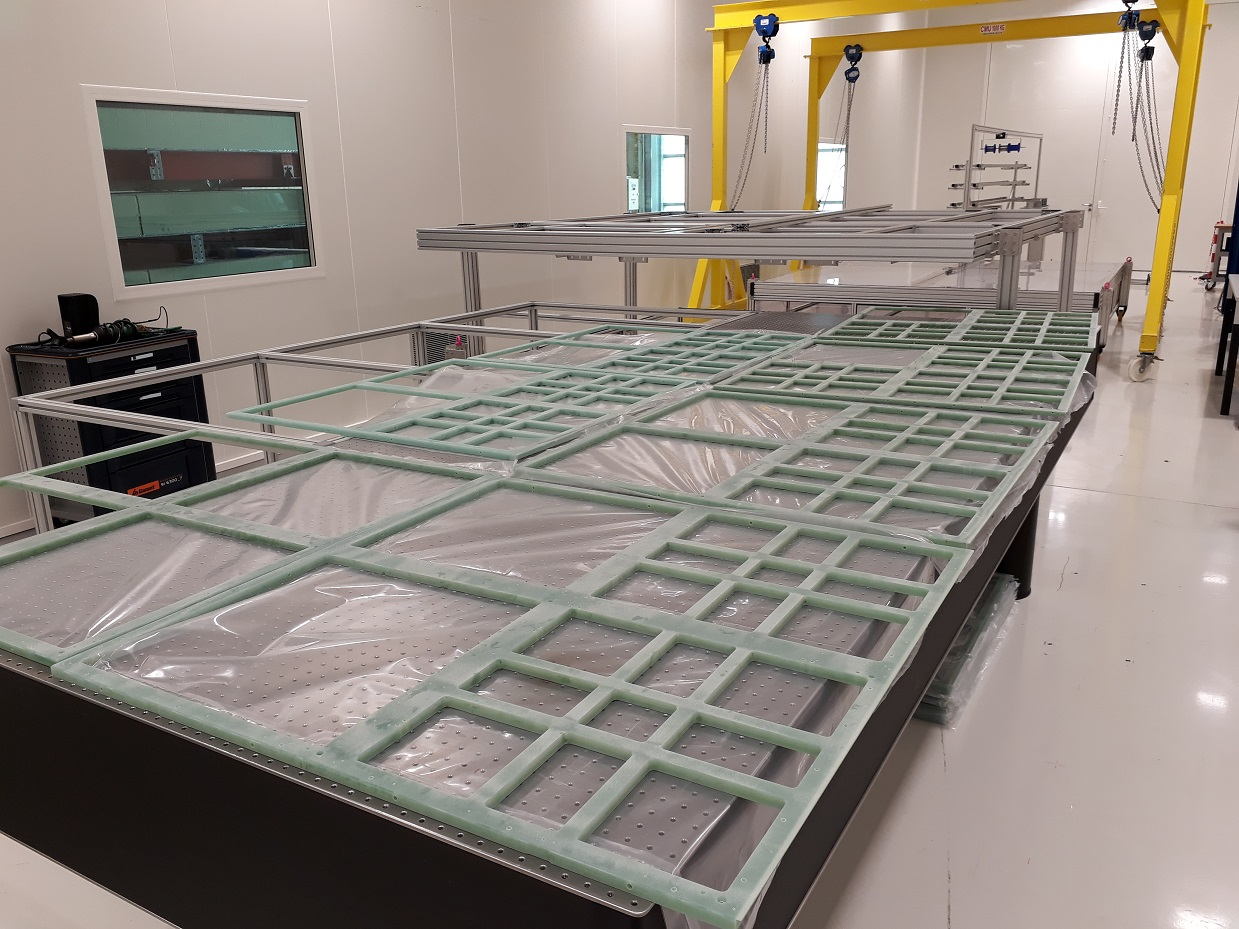
\includegraphics[width=0.4\textwidth]{20180426_160140redim.jpg}
\end{dunefigure}
Once ready, the planarity of the \dword{crp} is checked and adjusted using metrology and the decoupling systems.
All the components and instrumentation of the \dword{crp} are carefully checked, and the assembly is then packed in the transport box.
%% end new from DD

%An example of the assembly procedures performed for the \dword{crp}  construction in the clean room in Building 185 at CERN for \dword{pddp} can be seen at: \url{https://youtu.be/jcnJjlU-Cyc}.


%%%%%%%%%%%%%%%%%%%%%%%%%%%%%%%%%%%%%%%%%%%%%%%%%%%%%%%%%%%%%%%%%%%%
\section{Interfaces}
\label{sec:fddp-crp-intfc}

The main interfaces with the \dword{crp} are with the elements directly connected to them. The documents that describe the interfaces are referenced.
\begin{itemize}
\item The readout electronics  (DocDB 6751), concerning the cabling of the signal cables on the bottom part of the cold 
flange of the signal chimneys.  
\item The \dword{cisc} (DocDB 6760),  concerning the power supplies for the \dword{lem} and extraction grid, the cameras, \dword{led} ribbons, temperature sensors, and distance meters. All these devices go to the \dword{crp} instrumentation \fdth{}s. 

\item Drift \dword{hv} (DocDB 6754), at the level of design requirements. This includes the system for maintaining the proper distance between the top-most field shaping profile to the extraction grid in order to maintain the proper extraction field and to protect the contact between the two systems.
\end{itemize}

%%%%%%%%%%%%%%%%%%%%%%%%%%%%%%%%%%%
\subsection{TPC Electronics}
\label{sec:fddp-crp-intfc-elec}

The interface with the \dual TPC electronics is at the level of the bottom flanges of the \dwords{sftchimney} where the flat cables bringing the signals from the anodes are plugged in during the \dword{crp} installation in the cryostat. The system for %that allows 
pulsing the anode strips is installed by the \dword{crp} consortium %at the moment of 
concurrently with the \dword{crp} installations. %The strips calibration by using this system 
Calibration of the strips is then performed jointly by the two consortia.

%%%%%%%%%%%%%%%%%%%%%%%%%%%%%%%%%%%
\subsection{Instrumentation and HV Feedthrough Flanges}
\label{sec:fddp-crp-intfc-FT}
The \num{36} \dword{lem} modules of a \dword{crp} are supplied with \dword{hv} by \num{42} coaxial cables 
connecting the \fdth flange from the top of the cryostat to distribution boxes located on the \dword{crp} (Figure \ref{fig:CRP_DB}). Each cable (\num{20}\,AWG, \SI{50}{\ohm} Kapton\footnote{DuPont\texttrademark{} Kapton, polymide film,  E. I. du Pont de Nemours and Company,  \url{http://www.dupont.com/}.} insulated coaxial cable from ACCU-GLASS\footnote{ACCU-GLASS\texttrademark{}, \url{http://www.accu-glass.com/}.}) can sustain \SI{30}{kV} in air and has SHV plugs on each end in order to facilitate connections during the \dword{crp} installation.


There are six cables used for the \dword{lem} top electrodes and \num{36} cables for the bottom ones. Each of the coaxial cables for the \dword{lem} top electrodes is connected to a single distribution box. The latter contains a PCB that %allows to 
distributes \dword{hv} to six individual \dword{lem} modules with a \SI{500}{\mega\ohm} resistor in series for each 
\dword{lem} (Figure~\ref{fig:LEM_DB}). The \num{36} coaxial cables for the \dword{lem} bottom electrodes are connected in groups of four to nine distribution boxes. In this case, each \dword{hv} cable is directly linked to an individual \dword{lem} bottom electrode. In total, \num{72} output coaxial cables rated for \SI{10}{kV} (\num{26}\,AWG, \SI{50}{\ohm} Kapton insulated coaxial cable from ACCU-GLASS) are used to supply \dword{hv} to both electrodes of all \dword{lem} modules of a \dword{crp}. The grounding of each coaxial line is ensured by the \fdth flange down to about \SI{5}{cm} from the \dword{lem} final connection point via the PCB located inside each of the \num{15} distribution boxes. In this way, contributions from the \dword{hv} lines to the electronic noise is limited as much as possible. In order to avoid electrical discharges inside the distribution boxes, the latter are filled with Arathane\footnote{Arathane\texttrademark{} advanced polyurethane based adhesives, Huntsman Advanced Materials , \url{http://www.huntsman.com/advanced\_materials/a/Home}.} epoxy glue. Finally, the connections to the \dword{hv} contacts of the \dword{lem} modules are done via  Deutsch 6862-201-22278 female connectors and each of them is covered by a heat-shrink sleeve. 

\begin{dunefigure}
[\dword{lem} \dword{hv} distribution boxes mounted on a \dword{crp}]
{fig:CRP_DB} 
{\dword{lem} \dword{hv} distribution boxes mounted on a \dword{crp}. }
  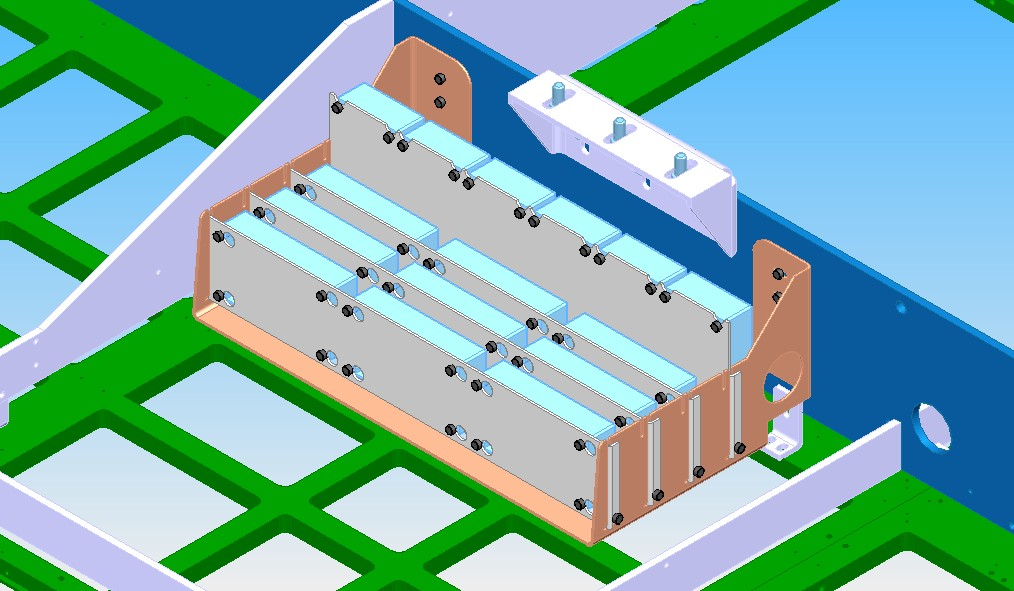
\includegraphics[width=.8\textwidth]{CRP_DB.jpg}
\end{dunefigure}


\begin{dunefigure}
[\dword{hv} distribution box for \dword{lem} top electrodes before filling]
{fig:LEM_DB} 
{\dword{hv} distribution box for \dword{lem} top electrodes before filling with ARATHANE glue. }
  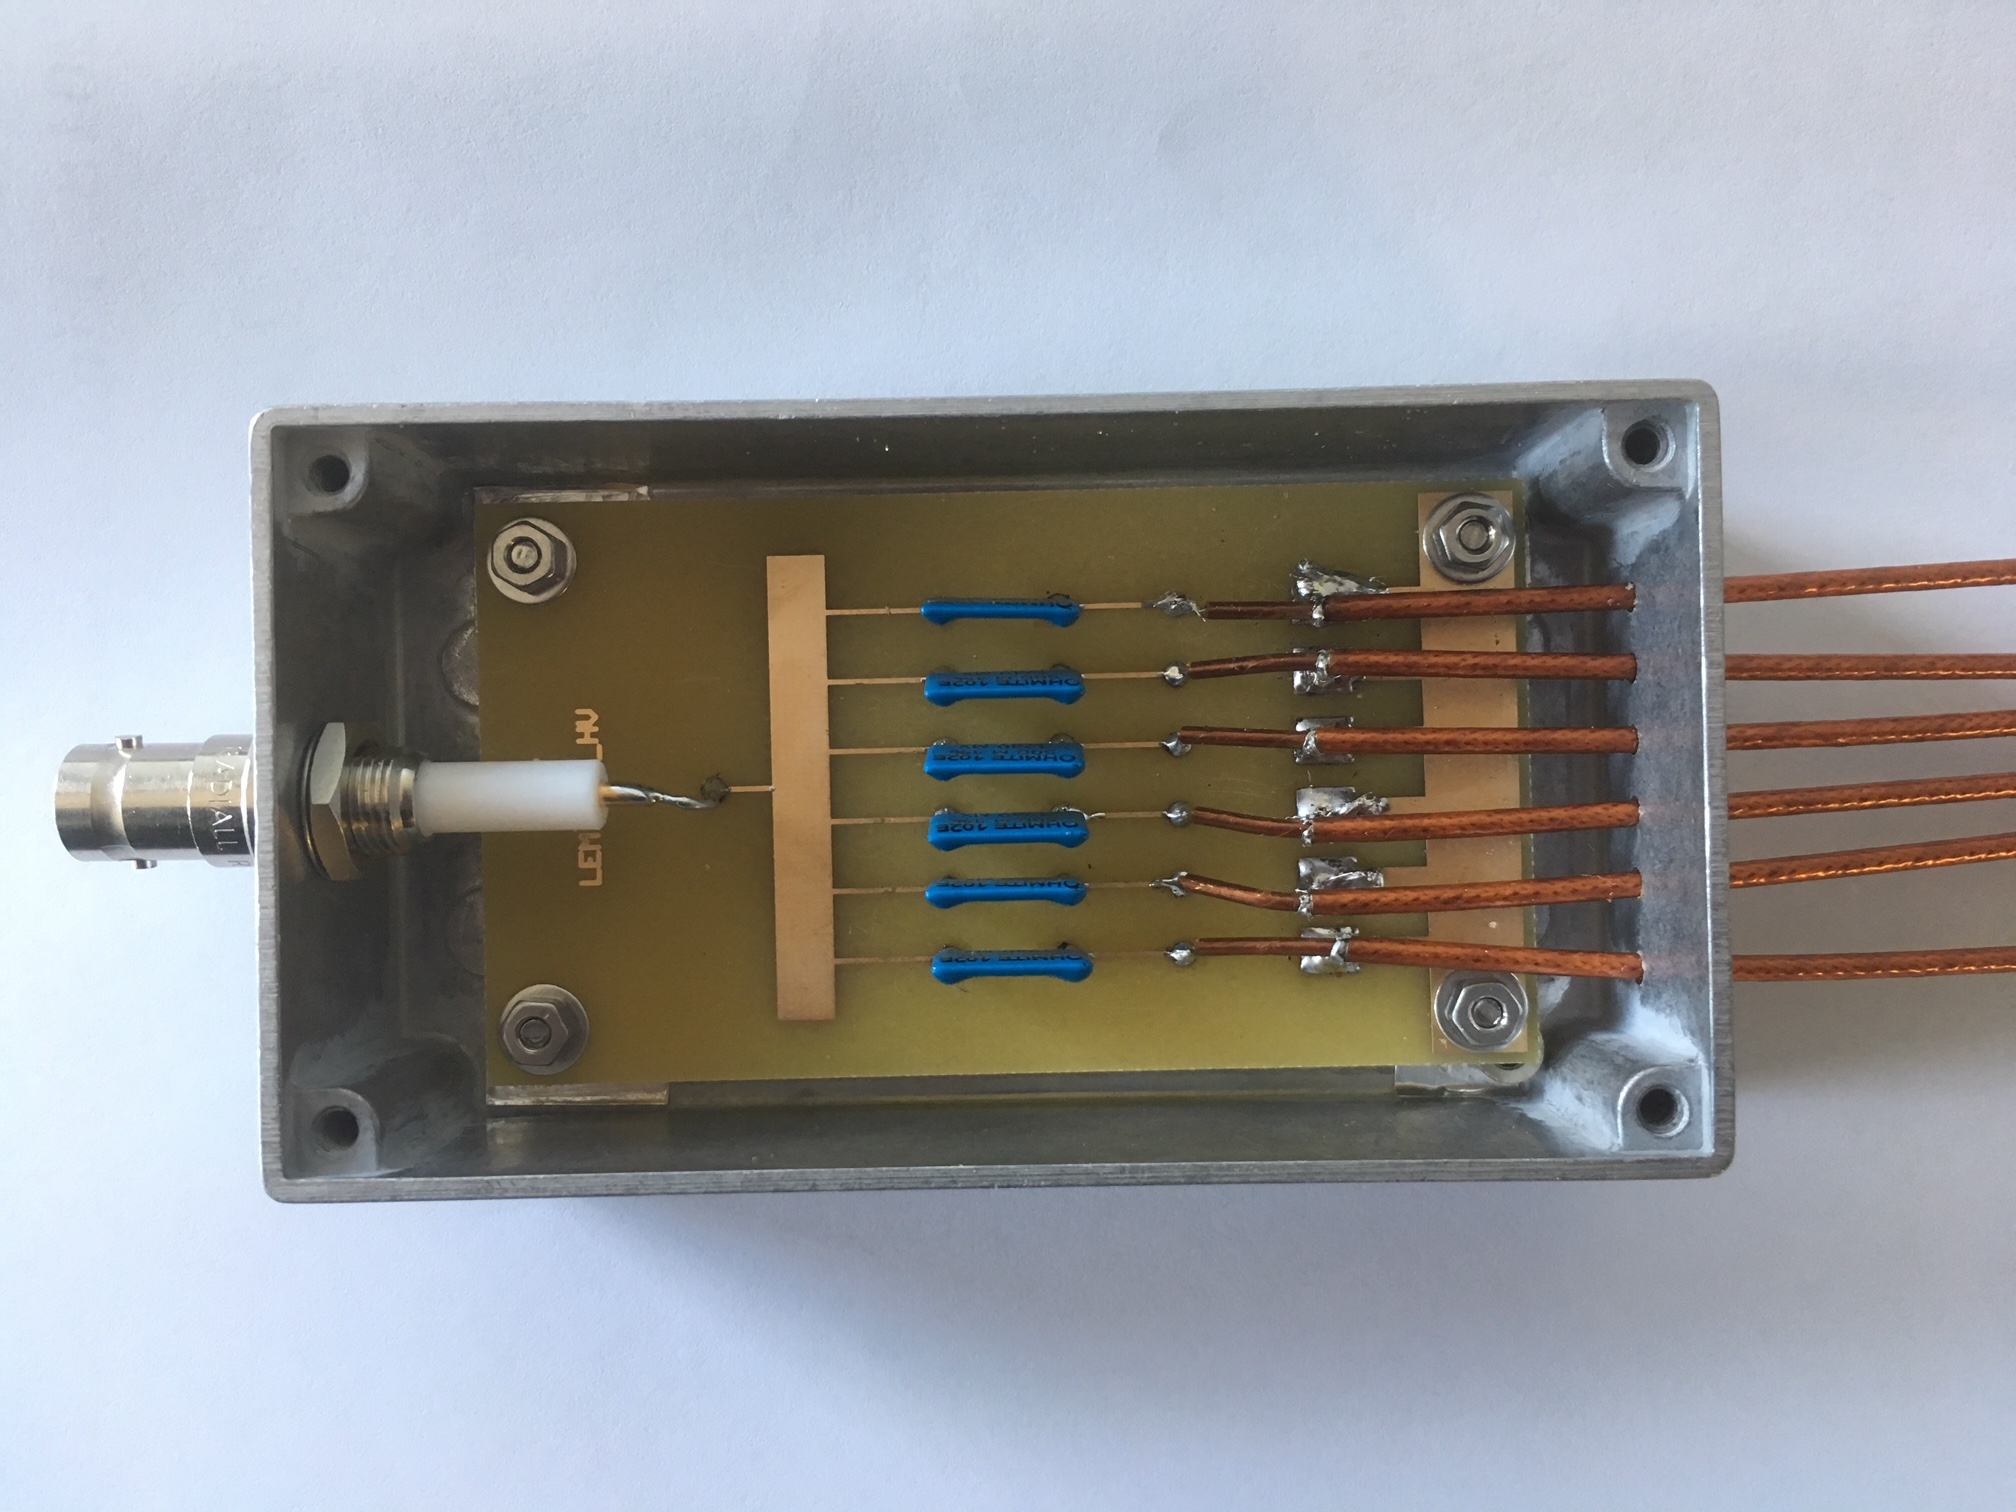
\includegraphics[width=.8\textwidth]{LEM_DB.jpeg}
\end{dunefigure}


%%%%%%%%%%%%%%%%%%%%%%%%%%%%%%%%%%% 
\subsection{Cryostat and Detector Support Structure}
\label{sec:fddp-crp-intfc-support}

The cryostat includes the dedicated penetrations for the hanging system of each \dword{crp}. Each penetration has a diameter of \SI{60}{mm}. The layout of the cryostat penetrations   matches the position of the hanging points on the \dword{crp} supporting structure. The penetration flanges and \dword{crp} suspension step motors are provided by the \dword{crp} consortium.

%%%%%%%%%%%%%%%%%%%%%%%%%%%%%%%%%%%
\subsection{HV and Slow Controls}
\label{sec:fddp-crp-intfc-HV-slowcontrol}

The interface with the slow controls includes:

\begin{itemize}
\item The procurement and control of the power supplies for the HV and grid \dword{lem} biasing;
\item The control of the \dword{crp} temperature probes and level meters;
\item The procurement and control of the \dword{crp} pulsing system (external to the cryostat);
\item The procurement of the instrumentation and \dword{hv} \fdth flanges;
\item The control of the \dword{crp} suspension step motors.
\end{itemize}

%%%%%%%%%%%%%%%%%%%%%%%%%%%%%%%%%%%%%%%%%%%%%%%%%%%%%%%%%%%%%%%%%%%%
\section{Installation, Integration and Commissioning}
\label{sec:fddp-crp-install}

The installation of the \dwords{crp} in the cryostat will be performed on a time span of eight months, following the installation of the signal chimneys, which will take three months. The signal chimneys must be present in order to %be able to 
connect the \dword{crp} signal flat cables. The suspension, instrumentation and \dword{hv} flanges must also be  installed prior to \dword{crp} installation. The installation of these flanges can be performed in parallel with the installation of the signal chimneys. 

The production of the \dwords{crp} will be performed before the installation, and the \dwords{crp} will be stored in temporary storage boxes at the production centers. During installation the already produced \dwords{crp} will be moved to the transportation boxes in order to be shipped to the ITF, which is used as a delivery destination buffer, and then immediately moved underground for installation. Given the installation rate of eight \dwords{crp}/month a set of \num{30} transportation boxes will ensure a sufficient turnover among the production sites and the installation site.

%\fixme{I can't make out when they leave the production site to go to the ITF, and when they leave ITF for installation at the 4850. It appears to be staggered.} DONE we cannot deliver directly to the mine, the ITF is the delivery destination

The installation procedure %foresees the operation from
plans for three two-person teams working in parallel inside the cryostat to %manage the installation of 3 
install three \dwords{crp} at a time. It is assumed that %of the order of 
approximately \num{1.3} weeks is needed for a team to prepare, survey, tune and cable a \dword{crp} in the  cryostat, and \num{35} working weeks for the overall installation of the \dptotcrp \dwords{crp}.

Once the three \dwords{crp} are ready to be lifted, three people are needed to manipulate the manual winches on the top of the cryostat for a few hours. This activity is expected to occur during the \num{1.3}-week period just before the cabling activity for the connection to the flanges.

%\fixme{Put here more details of the different steps for the underground installation/ positioning of the box, suspension of the \dword{crp}, cabling at height, etc .. and the associated tooling ! (not anne)}


%%% new from DD
The sequence of operations needed underground per \dword{crp} is similar to the one foreseen for \dword{pddp}  and is the following: 
\begin{enumerate}
\item A \dword{crp} module in its transport box is brought to the entrance of the cryostat.
\item The box is hung from the side of the insertion rail, and guided through the \dword{tco}.
\item  Inside the cryostat, the \dword{crp} is laid down horizontally, rolled below the \dwords{sftchimney}.
\item The structure is suspended from temporary cables going down from the chimney.
\item The transport box is dismounted and removed.
\item The \dword{crp} planarity is measured and tuned based on metrology survey.
\item The \dword{crp} is raised up with the manual winches, then the mechanical stop is assembled.
\item The \dword{crp} is lowered down  on the mechanical stop.
\item The cabling of the \dword{crp} patch panels to \dword{hv}, signal and slow control \fdth{}s is done.
\item The winch cable is disconnected  and the winch removed.
\item The bellows is compressed using special tooling.
\item The cable from the bellows is connected with a pin.
\item The compression tool is removed and the bellows attached.
\item The motor is inserted and screwed from the top.
\end{enumerate}
 

The assembly is then complete and operational.
The lateral and vertical alignment of the \dword{crp} is performed from the top of the cryostat with a SPFT translation mechanism, distance meter measurements and metrology.

The cabling activity is done  working at the nominal height position using elevating platforms. The access between two adjacent \dwords{crp} is done by staggering the altitude of the two modules by about \SI{20}{cm} allowing enough space to do the electrical connection. 
%%% end new from DD


%%%%%%%%%%%%%%%%%%%%%%%%%%%%%%%%%%%%
\subsection{Transport and Handling}
\label{sec:fddp-crp-install-transport}

The transportation boxes are sized (\num{3.5} $\times$ \num{3.5} $\times$ \SI{0.8}{m}) for the shafts and underground handling at \surf{}.
%\fixme{provide here the external envelope of the box(not anne)}
They are protected by a plastic layer that should be removed once the transportation box arrives at the clean area underground.
%\fixme{never heard of gray room area}
underground so that the box can be introduced into the cryostat in a clean state via the \dword{tco}. The transportation box is also essential for manipulating the \dword{crp} from the vertical orientation (i.e., for insertion in the \dword{tco}) to the horizontal orientation, required %in which the \dword{crp} should be
 prior to hanging it from the suspension system. Once the installation is complete the transportation boxes are wrapped again with a protective layer and shipped back to the production centers. 

%%%%%%%%%%%%%%%%%%%%%%%%%%%%%%%%%%%
\subsection{Calibration}
\label{sec:fddp-crp-install-calib}

The \dword{crp} calibration relies on a pulsing system that performs charge injection in the strips via \SI{1}{pF} capacitors. The pulse distribution system and related cabling, and the boards with the charge-injection capacitors are integrated  with the \dword{crp} at the time of the \dword{crp} assembly. At this time, this system is connected via flat cables to the instrumentation flange. A pulse distribution system external to the cryostat and  provided by the \dword{cisc} consortium ensures the signals feeding to the charge injection system. 
%\fixme{drives the system?} 
The information from the pulse calibration is then combined
%\fixme{combined?} 
with the one from the \dword{fe} electronics calibration and the one from the analysis of the reconstructed charged tracks in order to extract the overall calibration constants per channel.

%%%%%%%%%%%%%%%%%%%%%%%%%%%%%%%%%%%%%%%%%%%%%%%%%%%%%%%%%%%%%%%%%%%%
\section{Quality Control}
\label{sec:fddp-crp-qc}

Several quality control 
%\fixme{qa or qc?}
procedures are applied at the level of the \dword{lem} and anode production, as described in more detail in their corresponding sections. The components of the \dword{hv} distribution system are also individually tested. Continuity tests are performed at the time of the \dword{crp} assembly. The \dword{crp} geometry is also systematically surveyed as well as the tensioning of the grid wires. On a small subsample of the \dwords{crp} production, it will be also possible to perform cold-box testing by using the infrastructure set up at CERN for \dword{pddp}.


%%%%%%%%%%%%%%%%%%%%%%%%%%%%%%%%%%%%
%\subsection{Protection and Assembly (Local)}
%\label{sec:fddp-crp-qc-local}


%%%%%%%%%%%%%%%%%%%%%%%%%%%%%%%%%%%
%\subsection{Post-factory Installation (Remote)}
%\label{sec:fddp-crp-qc-remote}



%%%%%%%%%%%%%%%%%%%%%%%%%%%%%%%%%%%%%%%%%%%%%%%%%%%%%%%%%%%%%%%%%%%%
\section{Safety}
\label{sec:fddp-crp-safety}

Safety must be a central feature of all tasks performed by the \dword{crp} consortium.  All aspects of \dword{crp} construction, installation, and commissioning will adhere to procedures established by the DUNE Technical Coordinator and relevant host institutions. 

The \dword{crp} installation and operation does not present particular safety issues apart from working at heights %during the \dword{crp} installation 
for the connection of the  \dword{crp} cabling to the \dwords{sftchimney} and the instrumentation and \dword{hv} \fdth{}s.